% mnras_template.tex 
%
% LaTeX template for creating an MNRAS paper
%
% v3.0 released 14 May 2015
% (version numbers match those of mnras.cls)
%
% Copyright (C) Royal Astronomical Society 2015
% Authors:
% Keith T. Smith (Royal Astronomical Society)

% Change log
%
% v3.0 May 2015
%    Renamed to match the new package name
%    Version number matches mnras.cls
%    A few minor tweaks to wording
% v1.0 September 2013
%    Beta testing only - never publicly released
%    First version: a simple (ish) template for creating an MNRAS paper

%%%%%%%%%%%%%%%%%%%%%%%%%%%%%%%%%%%%%%%%%%%%%%%%%%
% Basic setup. Most papers should leave these options alone.
\documentclass[fleqn,usenatbib]{mnras}
\usepackage{cite}

% MNRAS is set in Times font. If you don't have this installed (most LaTeX
% installations will be fine) or prefer the old Computer Modern fonts, comment
% out the following line
\usepackage{newtxtext,newtxmath}
% Depending on your LaTeX fonts installation, you might get better results with one of these:
%\usepackage{mathptmx}
%\usepackage{txfonts}

% Use vector fonts, so it zooms properly in on-screen viewing software
% Don't change these lines unless you know what you are doing
\usepackage[T1]{fontenc}
\usepackage{ae,aecompl}
\usepackage{verbatim}

%%%%% AUTHORS - PLACE YOUR OWN PACKAGES HERE %%%%%

% Only include extra packages if you really need them. Common packages are:
\usepackage{graphicx}	% Including figure files
\usepackage{amsmath}	% Advanced maths commands
\usepackage{amssymb}	% Extra maths symbols
\usepackage{multicol}
\usepackage{multirow}
\usepackage{pdflscape}	% Landscape pages
\usepackage{amsmath} % or simply amstext
\newcommand{\angstrom}{\text{\normalfont\AA}}
\usepackage{color}

\usepackage{times}
\usepackage[space]{grffile}
\usepackage{cleveref}
\usepackage[normalem]{ulem}
\usepackage{natbib}
\usepackage{longtable}
\usepackage{hyperref}
\usepackage{comment}
\bibpunct{(}{)}{;}{a}{}{,}
\usepackage{pdflscape}	% Landscape pages
\usepackage{url}
\texorpdfstring


\newcommand{\sqcm}{cm$^{-2}$}
\newcommand{\alphaox}{$\alpha_\mathrm{ox}$}
\newcommand{\Gammaxray}{$\Gamma$}

\newcommand{\fek}{Fe~K$\alpha$}
\newcommand{\xmm}{{\em XMM-Newton}}
\newcommand{\nustar}{{\em NuSTAR }}
\newcommand{\chandra}{{\em Chandra}}
%\newcommand{\swift}{{\em Swift}}
\newcommand{\suzaku}{{\em Suzaku}}
\newcommand{\sax}{{\em BeppoSAX}}
\newcommand{\vla}{{\small VLA}}

\newcommand{\swift}{{\small \it Swift}}
\newcommand{\bat}{{\small {\it Swift}/BAT}}
\newcommand{\xrt}{{\small {\it Swift}/XRT}}
\newcommand{\uvot}{{\small {\it Swift}/UVOT}}



%%%%%%%%%%%%%%%%%%%%%%%%%%%%%%%%%%%%%%%%%%%%%%%%%%

%%%%% AUTHORS - PLACE YOUR OWN COMMANDS HERE %%%%%

% Please keep new commands to a minimum, and use \newcommand not \def to avoid
% overwriting existing commands. Example:
%\newcommand{\pcm}{\,cm$^{-2}$}	% per cm-squared

%%%%%%%%%%%%%%%%%%%%%%%%%%%%%%%%%%%%%%%%%%%%%%%%%%

%%%%%%%%%%%%%%%%%%% TITLE PAGE %%%%%%%%%%%%%%%%%%%
\graphicspath{{./}{pic/}}


% Title of the paper, and the short title which is used in the headers.
% Keep the title short and informative.
\title[Mrk1018]{Long-term and multi-wavelength evolution of a changing-look AGN Mrk 1018}

% The list of authors, and the short list which is used in the headers.
% If you need two or more lines of authors, add an extra line using \newauthor
\author[Bing Lyu et al.]{
Bing Lyu,$^{1,2}$
Zhen Yan,$^{2}$
Wenfei Yu,$^{2}$%\thanks{E-mail:wenfei@shao.ac.cn}
Qingwen Wu,$^{1}$\thanks{E-mail:qwwu@hust.edu.cn}
\\
% List of institutions
$^{1}$Huazhong University of Science and Technology, School of Physics, 1037 Luoyu Road, Wuhan, 430074, China\\
$^{2}$Shanghai Astronomical Observatory, CAS, 
Nandan Road 80, Shanghai, 200030, China\\
%$^{3}$Another Department, Different Institution, Street Address, City Postal Code, Country\\
%$^{4}$Department, Institution, Street Address, City Postal Code, Country
}

% These dates will be filled out by the publisher
\date{Accepted XXX. Received YYY; in original form ZZZ}

% Enter the current year, for the copyright statements etc.
\pubyear{2021}

% Don't change these lines
\begin{document}
\label{firstpage}
\pagerange{\pageref{firstpage}--\pageref{lastpage}}
\maketitle


\def\sectionautorefname{Section}
\def\subsectionautorefname{Section}


%%%%%%%%%%%%%%%%%%%%%%%%%%%%%%%%%%%%%%%%%%%%%%%%%%

%%%%%%%%%%%%%%%%% BODY OF PAPER %%%%%%%%%%%%%%%%%%
\begin{abstract}
The physical mechanism for triggering the changing-look phenomenon in active galactic nuclei (AGNs) is still unclear. We explore this issue based on the multi-wavelength spectral and flux variations for a changing-look AGN Mrk~1018 with long-term observations in the X-ray, optical/ultraviolet(UV), and radio bands. %We find that the optical/UV emission slightly decreases while the X-ray emission keeps roughly unchanged in type 1 phase before 2010. 
Both the optical and the X-ray emission experience rapid decay in changing-look phase during 2010--2015, where a re-flare appears in the optical/UV and X-ray bands. The 5 GHz radio flux decreases by $\sim 20$\% in type 1.9 phase during 2016--2017. We find both X-ray photon index ($\Gamma$) and the optical-to-X-ray spectral index (\alphaox\,) are anti-correlated with the Eddington scaled 2--10~keV X-ray luminosity ($L_\mathrm{X}/L_\mathrm{Edd}$) in the type 1.9 phase. However, the type 1 phase deviates from these two anti-correlations, which suggests that the change of broad emission lines might be regulated by the evolution of accretion disk (e.g., disappearing of the inner cold disk in the type 1.9 phase). %The radio and X-ray luminosity follow a roughly flat correlation for Mrk 1018, which is much shallower than that found in low-luminosity AGNs and low-hard state X-ray binaries.
\end{abstract}

\begin{keywords}
galaxies: active -- galaxies: Seyfert -- individual: Mrk 1018 
\end{keywords}
\section{Introduction}\label{sec:intro}
%Seyfert 1.9 (S1.9) is a Seyfert 1
%\textcolor{red}{}

\textcolor{red}{Type 1 and type 2 of Seyfert galaxies are classified based on the widths of optical spectral emission lines from the nuclei.} Type 1 Seyfert galaxies show both broad lines ($>$ 1000 $ \rm{km}\, \rm{s}^{-1}$) and narrow lines ($<$ 1000 $ \rm{km}\, \rm{s}^{-1}$), while type 2 Seyfert galaxies show only narrow lines. In the active galactic nucleus (AGN) unification model \citep[e.g.][]{1993ARA&A..31..473A}, A Seyfert 1  is face-on to the observer with broad lines visible to us, while Seyfert 2 is edge-on with broad line region blocked by the torus. The sub-classes (e.g. Seyfert 1.5, 1.8 and 1.9) are also introduced \citep[see ][]{1976MNRAS.176P..61O,1981ApJ...249..462O} based on the emission line width and relative strength of the broad-line to the narrow-line. For example, there are only broad H$\alpha$ lines in Seyfert 1.9 (S1.9), broad H$\alpha$ lines plus very weak broad H$\beta$ lines in Seyfert 1.8 (S1.8) and comparable H$\alpha$ and H$\beta$ lines in Seyfert 1.5 (S1.5). In recent years, several tens of changing-look AGNs (CL-AGNs hereafter) have been discovered within a timescale of decades or years \citep[e.g.][]{2014ApJ...796..134D,2014ApJ...788...48S,2015ApJ...800..144L,2016A&A...593L...8M,2016MNRAS.461.1927P,2019MNRAS.486..123R,2020ApJ...890L..29A,2020ApJ...901....1W,2020A&A...638A..91K}, or even months \citep[e.g.][]{2018arXiv181103694K,2019ApJ...883...94T}, which show disappearance/appearance of broad emission lines. It should be noted that the ``changing-look'' was originally used to describe the change of AGNs from Compton-thick to Compton-thin (or vice versa) based on the X-ray observations \citep[e.g.][]{2003MNRAS.342..422M}. 

The physical mechanisms of the changing-look phenomena are still under debate. On the one hand, the ``changing-look'' can be attributed to variable obscuration, such as obscuring material moving in or moving out from our line of sight \citep[e.g.][]{2013MNRAS.436.1615M,2014MNRAS.443.2862A,2015ApJ...815...55R,2018MNRAS.481.2470T}, where the intrinsic radiation spectrum is unchanged. On the other hand, the change may be triggered by the variation of intrinsic radiation \citep[e.g., the change of accretion disk,][]{1984MNRAS.211P..33P,2014MNRAS.438.3340E}. There are also many evidences for the variations in different wavebands in CL-AGNs, where the variations in radio \citep[e.g.][]{2016MNRAS.460..304K}, infrared \citep[e.g.][]{2017ApJ...846L...7S,2018ApJ...864...27S}, optical/ultraviolet \citep[e.g.][]{2019ApJ...885...44D} and X-ray \citep[e.g.][]{2016MNRAS.461.1927P,2019MNRAS.483L..88P,2020ApJ...898L...1R} bands are also reported when the AGNs change from type 1(2) to type 2(1). It is also found that the absorption is roughly unchanged in some CL-AGNs even the X-ray spectra varied a lot \citep[e.g.][]{2016A&A...593L...9H,2020ApJ...890L..29A,2020ApJ...901....1W}. Therefore, the intrinsic mechanism for the ``changing-look'' of AGNs is quite unclear. The high-cadence monitoring observations of the CL-AGNs can shed light on this issue. 

The Seyfert galaxy Mrk~1018 at $z=0.042$ has undergone a full cycle with twice type transitions during the past 40 years. It transited from S1.9 to S1 between 1979 and 1984 \citep{1986ApJ...311..135C} and returned to S1.9 after 30 years as a S1 \citep[see also][]{2016A&A...593L...8M,2016A&A...593L...9H,2017A&A...607L...9K}. The recent optical spectroscopic observations reveal that Mrk~1018 is a type 1 AGN in 2009 January, 2009 December and 2010 December and a type 1.9 AGN in 2015 January \citep{2016A&A...593L...8M,2018ApJ...861...51K}. The latest spectroscopic observation of Mrk~1018 in 2019 October shows a faint broad H$\beta$ line component in \citet{2020A&A...644L...5H}, which is similar to the type 1.9 spectrum as reported in \citet[][]{2016A&A...593L...8M}. Between 2010 and 2016, the optical and X-ray flux decrease by a factor of $\sim$ 17 and $\sim$ 8 \citep{2016A&A...593L...9H}, respectively, where the intrinsic absorption is negligible based on the X-ray observations. The spectroscopic observations during this period are absent, which may correspond to a changing-look phase.

The multi-wavelength and long-term variability of the CL-AGNs can improve us to understand the physical mechanisms for the CL behavior. In this work, we try to explore this issue based on performing an extensive data analysis for a CL-AGN of Mrk~1018 in radio band, optical/ultraviolet and X-ray bands. This paper is presented as as follows: In \autoref{sec:data}, we describe the observations and the data reduction in different wavebands. In \autoref{sec:result}, we present the multi-wavelength observational results. In \autoref{sec:discussion}, we discuss possible physics behind the observational results. Finally, we summarize our results in \autoref{sec:conclusion}. Throughout this work, we use a flat $\Lambda-$CDM cosmological model with $\Omega_{\rm{M}}$=0.27, $\Omega_\Lambda=$0.73 and a Hubble constant of 70 km s$^{-1}$ Mpc$^{-1}$. We adopt the luminosity distance $d_{\rm{L}}=176 $ Mpc and the black hole (BH) mass measurement $\log(M_{\rm{BH}}/M_{\odot})=7.84$ \citep{2017MNRAS.472.3492E,2018MNRAS.480.3898N} for Mrk~1018. 


%\textcolor{red}{Observations in different wavelengths have covered the timeline before and after the recent changing-look of Mrk~1018 for exploring the possible physical mechanism for the changing-look behavior.


%supports that the "changing-look" is driven by the activity of the central engine.
% 2016MNRAS.457..389M,2016ApJ...826..188R,2020MNRAS.491.4925G, quasar
% 2019ApJ...874....8M quasar candidate
 % 2018ApJ...864...27S, mid-infrared
 % 2019MNRAS.486..123R The reappearance of the broad emission lines
 % \citep[e.g.][]{}.





%\clearpage
\section{Data reduction and analysis}\label{sec:data}
\subsection{X-ray data analysis}
We analyse the public archival data of \swift, \xmm, \chandra ~and \nustar during the period between 2005 and 2019. We use the cosmic abundances of \citet{2000ApJ...542..914W} and the photoelectric absorption cross sections from \citet{1995A&AS..109..125V}. All the X-ray spectra are fitted by an absorbed power-law model  \texttt{tbabs*zpowerlw} with the absorption by the Galactic hydrogen fixed at $N_{\rm{HI,Gal}}=2.43 \,\times \,10^{20}\, \rm{cm}^{-2}$ \citep[][]{2005A&A...440..775K} since no intrinsic absorption beyond Galactic is detected \citep[see][]{2016A&A...593L...9H,2017A&A...607L...9K}. The 2--10~keV flux are calculated by {\it cflux} component within {\tt XSPEC} (v12.10). The observation information and best-fitting parameters including photon index ($\Gamma$), unabsorbed flux in 2--10~keV ($F_{\rm{2-10~keV}}$) are listed in \autoref{tab:tablexray}. The long-term X-ray light curve in 2--10~keV band is shown in the top panel of \autoref{fig:multi-lc-secondaxis}.


\subsubsection{\xrt\,}
\label{data-xrt}
The X-ray telescope (XRT) on board \swift\, has the highest cadence monitoring observations of Mrk~1018 in the X-ray band, especially after 2015. We reprocess the archive data of \xrt\, observations performed in photon counting mode with {\scriptsize XRTPIPELINE}. The source region is a circle centered at the nucleus of Mrk 1018, the radius of which is determined by the count rate of each observation according to \citet{2009MNRAS.397.1177E}. We use {\scriptsize XSELECT} to extract the source and background spectra. The spectra are grouped by the a minimum of one count per bin. The XRT spectra of Mrk~1018 in the 0.5--10~keV range are fitted using the Bayesian X-ray Analysis (BXA)\footnote{\url{http://johannesbuchner.github.io/BXA/index.html}} method.  %'range' is right


\subsubsection{\chandra/ACIS-S}
We extract the ACIS-S spectra with CIAO (v4.12) and {\tt CALDB} (v4.9.1). For the observation in November of 2010 (ObsID 12868), which is affected by the pile-up effect, we adopt the fitting results from \citet{2016A&A...593L...9H} which excluded the bright pixels and corrected the photon loss for this observation. The other observations are extracted from a 3$\arcsec$ radius circle and the background spectra are extracted from an annulus with 5$\arcsec$ inner radius and 15$\arcsec$ outer radius \citep[see also][]{2017ApJ...840...11L}. Then the spectra are grouped by a minimum of 20 counts per bin and fitted in the 0.5--8~keV range. 



\subsubsection{$XMM-Newton$/EPIC-PN }
We analyse the archival data sets of Mrk~1018 derived by the EPIC-PN on board \xmm\,. The source is observed in 2005 (ObsID 201090201) and 2008 (ObsID 554920301). We reduce the PN data with {\scriptsize EPPROC} in \texttt{SAS-16.1.0}. The source and background regions are a 40$''$ and 60$''$ radius circle, respectively. Each spectrum is grouped by a minimum of 30 counts per bin and fitted in the 2--10~keV range. 


\subsubsection{$NuSTAR$}
We analyse the archival data sets of Mrk~1018 on board \nustar, which are reduced through the {\scriptsize NUPIPELINE} task of the {\scriptsize NUSTARDAS} package. The source region is a 50$''$ radius circle at the center of the source, and the background is extracted from the blank region. Each spectrum is grouped by a minimum of 30 counts per bin and fitted in the 3--79~keV range.

\subsection{\uvot\,data analysis}
\label{sec:uvot}
%f_uuu=(constants.c/(3465*units.AA)).to(u.Hz).value
%f_uw1=(constants.c/(2600*units.AA)).to(u.Hz).value
%f_um2=(constants.c/(2246*units.AA)).to(u.Hz).value
%f_uw2=(constants.c/(1928*units.AA)).to(u.Hz).value
There are six filters in the optical/UV band of \uvot, which are V, B, U, UVW1, UVM2, and UVW2 bands. We use the tool \textit{uvotsource} to do the aperture photometry for each filter of all the observations. The source aperture radius is 5$\arcsec$ and the background is chosen in a blank region with a much larger radius. According to the results in \citet{2018MNRAS.480.3898N}, the emission of the host galaxy is dominated in the V and the B band, we then discard all the results of the V and the B band. 

In order to correct the Galactic extinction, we adopt $E(B-V) = 0.036$ \citep[see][]{2018MNRAS.480.3898N} and $R_{V}=3.1$ for the Galactic extinction and calculate the values of $A_{\lambda}$ for U, UVW1, UVM2, and UVW2 band are  0.18, 0.25, 0.35 and 0.31 assuming the extinction model of \citet{2007ApJ...663..320F}. In order to estimate the intrinsic optical/UV flux from the nucleus, we subtract the contribution from the host galaxy, which is estimated from the broadband spectral modeling result in \citet{2018MNRAS.480.3898N}. The results of the long-term optical and UV light curves from \uvot\, are shown in the middle panel of \autoref{fig:multi-lc-secondaxis} and listed in \autoref{tab:tableuvot}.




\subsection{Radio data analysis}
\label{subsec:vla}
%\subsubsection{VLA}
We analyse the archival data of Very Large Array (VLA) observations for Mrk~1018 with \textsc{casa} version 5.3.0 \citep{2007ASPC..376..127M}. For the reduction of the pre-EVLA upgrade VLA data (VLA, project ID: AU0020, AB0476, AB0540, and AB0878), we manually flag and calibrate the data, then clean the image following the instruction\footnote{\url{https://casaguides.nrao.edu/index.php/VLA_5_GHz_continuum_survey_of_Seyfert_galaxies}}. For the new Karl G. Jansky Very Large Array data (JVLA, project ID: 16A-444, 16B-084, and 18B-245), calibrations are performed using script {EVLA\_pipeline1.4.2}\footnote{\url{https://science.nrao.edu/facilities/vla/data-processing/pipeline/scripted-pipeline}}. Different bands are split into different MS files after checking the radio frequency interference and calibration. Then the source is imaged using {\scriptsize TCLEAN} method and integrated flux is estimated via \textsc{imfit} task. The uncertainty of flux density is calculated from $\sigma_\mathrm{S}=\sqrt{(rms)^2+(0.05\times S)^2}$, where $5 \%$ absolute flux error is taken into account, except for the quick look image result in epoch 1 of {\em VLA Sky Survey (VLASS1.1)}, where $15 \%$ system error is considered according to the {\em VLASS Epoch 1 Quick Look Users Guide} \footnote{\url{https://science.nrao.edu/science/surveys/vlass/vlass-epoch-1-quick-look-users-guide}}. The imaging results are listed in Table.~\ref{tab:tableradio}. 


To compare between different periods and keep consistent with the radio and X-ray correlation in literature, we convert the radio flux to 5 GHz if it was observed at other wavebands using $S_v \propto v^{-\alpha_\mathrm{R}}$. The radio flux density of Mrk~1018 in the same band varied little before 2015, so we assume the radio spectral index also remains constant during this period. We calculate the $\alpha_\mathrm{L-X} =0.3 \pm 0.08$ using the observations on 50970 MJD (X band) and 52490 MJD (L band), then convert the flux densities at other bands to 5 GHz during this period (see \autoref{tab:tableradio}). There is one observation with two bands (C and X) available on MJD 57481, the $\alpha_\mathrm{C-X} =0.25\pm0.1$ is consistent within uncertainties with previous measured $\alpha_\mathrm{L-X}$. We then use this value to convert the flux densities of other bands to 5 GHz after MJD 57481. The estimated radio light curve at 5 GHz after 2005 is present in the bottom panel of \autoref{fig:multi-lc-secondaxis}.


\section{Results}
\label{sec:result}
\subsection{Multi-wavelength light curves}
\label{sec:multi-lc}%,fig:x-ray-uv-lc-rp-secondaxis,fig:radio-lc
Multi-wavelength light curves of Mrk~1018 are presented in \autoref{fig:multi-lc-secondaxis}. Between 2005 and 2010, when Mrk~1018 stayed in the bright type 1 phase, the X-ray flux was roughly unchanged. The optical/UV flux showed a slight decline by a factor $\sim 1.4 $ during 2005--2007. 

Between 2010 and 2015, both the optical/UV and the X-ray flux showed rapid decay \citep[see also ][]{2016A&A...593L...8M,2016A&A...593L...9H}, and Mrk~1018 changed from type 1 into type 1.9. The optical/UV and X-ray flux declined by a factor of $\sim 17$ and $\sim 7.5$, respectively. 

We find a re-flare (around 2013-2014) during the decay phase, while the amplitude of X-ray variation is higher than those in optical/UV bands (see \autoref{fig:multi-lc-secondaxis}, the X-ray flux increase by a factor $\sim 3$ within $\sim$ 100 days then decrease by a factor of $\sim 4.2$. The optical/UV flux increase by a factor of $\sim 1.5$ within $\sim$ 100 days then decrease by a factor of $\sim 3.8$.). After 2015, the source went into the faint type 1.9 phase. The X-ray showed stronger variability ($\sim $ 14 \%) than optical/UV bands ($\sim $ 6 \%) during the type 1.9 phase in 2018.  

The 5 GHz radio flux did not decline during the decay of X-ray and optical/UV emission between 2010 and 2015 and, however, it decreased by $\sim 20$ \% in the type 1.9 phase during 2016--2017 (see \autoref{fig:multi-lc-secondaxis}).



\begin{figure*}
\centering
	% To include a figure from a file named example.*
	% Allowable file formats are eps or ps if compiling using latex
	% or pdf, png, jpg if compiling using pdflatex
	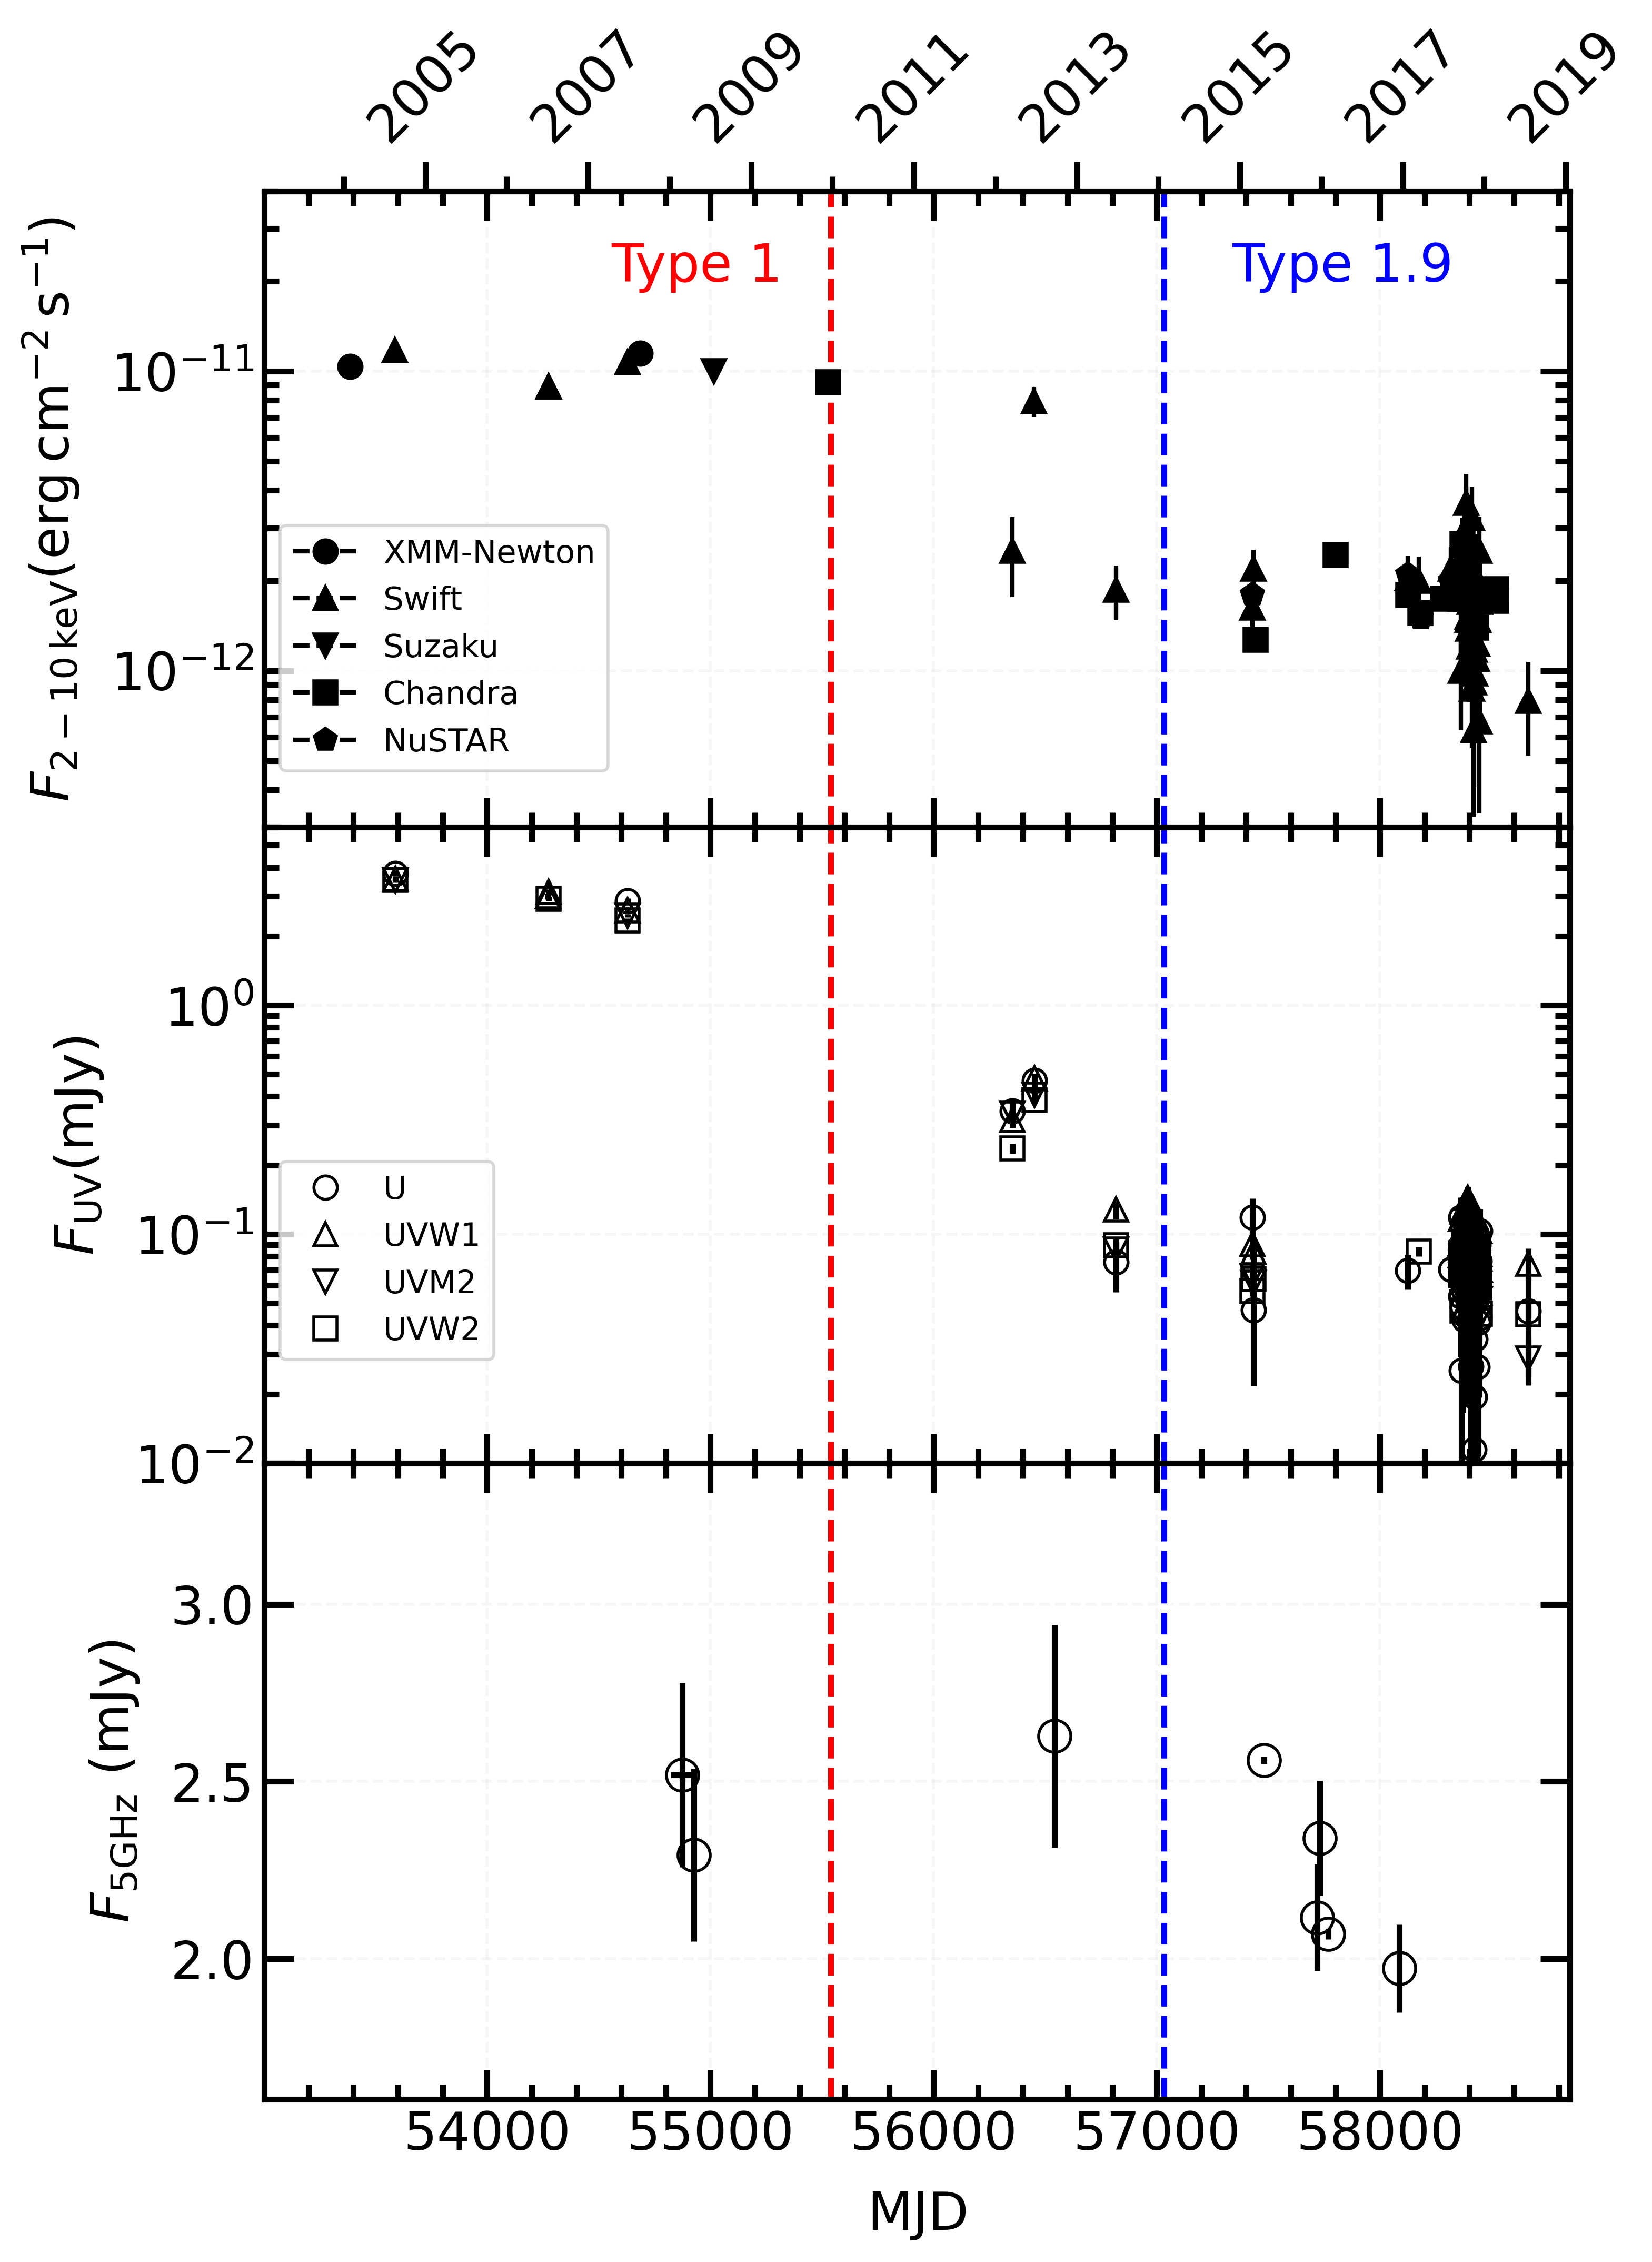
\includegraphics[width=0.9\textwidth]{./pic/subplots-xrt_uvot-radio-second.png}
    \caption{Multi-wavelength light curves of Mrk~1018 between 2005 and 2019. Red and blue vertical dashed lines represent the timeline of optical spectroscopic confirmation at type 1 and type 1.9, respectively. A re-flare during the changing-look phase is found in both the X-ray and the optical/UV bands.}
    \label{fig:multi-lc-secondaxis}
\end{figure*}

\subsection{Time lag between X-ray and UV variations}
Between 2018 August and 2018 November, \swift\, executed a rich monitoring campaign on Mrk~1018 (48 visits within 84 days). In order to examine the correlation between X-ray and UV flux variations during this period, we use the interpolation cross correlation function \citep[ICCF;][]{1998PASP..110..660P} with a time lag ($\tau$) range of 0--40 days (around half the overlap). The interpolation time step of 1 day are both applied to X-ray and UV light curves. The flux randomization and random subset selection methods are employed with 10000 realizations in the Monte Carlo simulation to estimate the centroid time lag and the error \footnote{The code \texttt{pyCCF} is available in \url{http://ascl.net/code/v/1868}}. We find a candidate time lag between X-ray and UVW1 band at $\tau \sim 18.1 ^{+6.5}_{-10.1} $ days (X-ray lead UV) with a correlation coefficient of 0.46 and a $p$-value of 1.3$\times10^{-3}$.

We use the \texttt{JAVELIN} algorithm \citep[][]{2011ApJ...735...80Z,2013ApJ...765..106Z} to further examine the time lag that we estimate through the ICCF method. The \texttt{JAVELIN} approach fits the light curves using a damped random walk (DRW) model, convolves them with a top-hat transfer function (TF), and aligns them to recover the time lag and other parameters (such as the amplitude and timescale of the DRW process, the height and width ($w$) of the top-hat transfer function) with the Monte Carlo method. We first restrict the range of time lag $\tau$ and the $w$ to be 0--40 days. We find a time lag between X-ray and UVW1 band at $\tau \sim 21.4^{+2.2}_{-2.8}$, which is consistent with the results through ICCF method. We find two peaks of the posterior likelihood distribution of $\tau$ ($\sim$ 20 and 32 days) between X-ray and UVM2 band, while the peak at $\sim$ 32 days is higher than that in $\sim$ 20 days. This result does not agree with the ICCF method. So we perform an additional simulation and restrict the range $w$ to be 15--40 days. We find only one peak of the posterior likelihood distribution of $\tau$ at $\sim$ 23 days. 

We estimate the time lag on a magnitude of $\sim $ 20 days between X-ray and UV bands at the 5\% significance level. We cannot distinguish the inter-band time lags in UV bands within errors. We list the detailed time lag analysis results in \autoref{tab:tablelag}.
%\begin{table}
\renewcommand{\arraystretch}{1.5}
\centering
\caption{{\bf Detected time lag $\tau$ of the UV variations behind the X-ray.} The X-ray band is taken as the reference. Errors refer to $1\sigma$ uncertainties.}
\label{tab:tablelag}
\begin{tabular}{lcccccr}
\hline
\hline
 band & method & $\tau$ & correlation coefficient & $p$-value   \\ 
      &        &  [day] &                         &             \\ \hline
U     & ICCF &  $13.4 ^{+17}_{-6} $ & 0.40 & 3.8e-3  \\
UVW1  & ICCF &  $18.1 ^{+6.5}_{-10.1} $ & 0.46 & 1.3e-3 \\
UVM2  & ICCF &  $21.0 ^{+8}_{-5.1} $ & 0.50 & 1.4e-3 \\
UVW2  & ICCF &  $21.0 ^{+6.5}_{-14} $ & 0.37 & 1.7e-2 \\
\hline \hline
band & method & $\tau$ & $w$ range &  $w$  \\ 
     &        &  [day] & [day]  &    [day]  \\ \hline 
U     & \texttt{JAVELIN} &  $ 14.7^{+10.4}_{-8.6} $ & 0--40 & $16.5 ^{+13.4}_{-10.6} $ \\
UVW1  & \texttt{JAVELIN} &  $ 21.4 ^{+2.2}_{-2.8} $  & 0--40 & $9.3 ^{+8.2}_{-5.7} $  \\
UVM2  & \texttt{JAVELIN} &  $ 23.4^{+7.3}_{-9.6} $  & 15--40 &  $ 25.1^{+8.7}_{-7.2} $  \\
UVW2  & \texttt{JAVELIN} &  $ 20.9 ^{+11.4}_{-13.2} $  & 0--40&  $ 12.7 ^{+16.9}_{-10.4} $ \\
\hline \hline
\end{tabular}   
\end{table}


\begin{table}
\renewcommand{\arraystretch}{1.5}
\centering
\caption{{\bf Detected time lag $\tau$ of the UV variations behind the X-ray.} The X-ray band is taken as the reference. Errors refer to $1\sigma$ uncertainties.}
\label{tab:tablelag}
\begin{tabular}{lcccccr}
\hline
\hline
 band & method & $\tau$ & correlation coefficient & $p$-value   \\ 
      &        &  [day] &                         &             \\ \hline
U     & ICCF &  $13.4 ^{+17}_{-6} $ & 0.40 & 3.8e-3  \\
UVW1  & ICCF &  $18.1 ^{+6.5}_{-10.1} $ & 0.46 & 1.3e-3 \\
UVM2  & ICCF &  $21.0 ^{+8}_{-5.1} $ & 0.50 & 1.4e-3 \\
UVW2  & ICCF &  $21.0 ^{+6.5}_{-14} $ & 0.37 & 1.7e-2 \\
\hline \hline
band & method & $\tau$ & $w$ range &  $w$  \\ 
     &        &  [day] & [day]  &    [day]  \\ \hline 
U     & \texttt{JAVELIN} &  $ 14.7^{+10.4}_{-8.6} $ & 0--40 & $16.5 ^{+13.4}_{-10.6} $ \\
UVW1  & \texttt{JAVELIN} &  $ 21.4 ^{+2.2}_{-2.8} $  & 0--40 & $9.3 ^{+8.2}_{-5.7} $  \\
UVM2  & \texttt{JAVELIN} &  $ 23.4^{+7.3}_{-9.6} $  & 15--40 &  $ 25.1^{+8.7}_{-7.2} $  \\
UVW2  & \texttt{JAVELIN} &  $ 20.9 ^{+11.4}_{-13.2} $  & 0--40&  $ 12.7 ^{+16.9}_{-10.4} $ \\
\hline \hline
\end{tabular}   
\end{table}




%\Cref{}
%Radio


\subsection{$\Gamma$-$L_\mathrm{X}/L_\mathrm{Edd}$ and \alphaox- $L_\mathrm{X}/L_\mathrm{Edd}$ correlation}\label{subsec:xray-uv}
We present the $\Gamma$-$\log{L_\mathrm{X}/L_\mathrm{Edd}}$ correlation of Mrk~1018 in \autoref{fig:xrayappendgood-Lrateandg-tmap}, where only the data of \xrt\, are adopted to avoid the discrepancies of different instruments. We find an evident negative correlation between the photon index and the Eddington-scaled X-ray luminosity in the type 1.9 phase, where the Spearman correlation coefficient is $-0.63$ ($p=5.1\times10^{-7}$). The data in the type 1 phase and the re-flare apparently deviate from the negative correlation (see \autoref{fig:xrayappendgood-Lrateandg-tmap}). 

The correlation of $\alpha_{\rm ox}-\log{L_\mathrm{X}/L_\mathrm{Edd}}$ is also explored in \autoref{fig:alpha_ox_lx}. We calculate the $\alpha_{\rm ox}$ according to the \autoref{definition_alpha_ox}. The $L_\mathrm{UVW1}$ is derived from UVW1 filter of the \uvot\ with central wavelength {2600{$\angstrom$}} and full-width at half max of $\sim 683\angstrom$ \citep{2008MNRAS.383..627P}. The $L_\mathrm{2~ keV}$ is calculated according to \autoref{definition_f2eV}, where the $L_\mathrm{2-10~ keV}$ and photon index $\Gamma$ are derived from X-ray spectra fitting. 
%\begin{equation}
%\alpha_{OX}  = - \frac{\log(\lambda F_{2500 \angstrom}/\nu F_{2keV})}{\log(\nu_{ 2500 \angstrom }/\nu_{2keV})}+1
%\end{equation}
\begin{equation}
\alpha_\mathrm{ox} = \frac{\log (L_\mathrm{UVW1} / L_\mathrm{2keV} )} {\log (\nu_\mathrm{2keV} /  \nu_\mathrm{UVW1} )}=0.384\times {\log (L_\mathrm{UVW1} / L_\mathrm{2keV} )}
\label{definition_alpha_ox}
\end{equation}
%and the $L_\mathrm{2keV}$ is estimated from
\begin{eqnarray}
\large{
L_\mathrm{2~keV}= 
\begin{cases}\displaystyle\frac{L_\mathrm{2-10~ keV} (2-\Gamma)}{\nu_\mathrm{2~keV} \times (5^{2-\Gamma}-1)} \quad &, 
\Gamma \neq 2 \\ 
\displaystyle\frac{L_\mathrm{2-10~ keV}}{\nu_\mathrm{2~keV} \times \mathrm{ln} 5}\quad  &, \Gamma = 2
\end{cases} }
\label{definition_f2eV}
\end{eqnarray} 
The \alphaox\, and $\log{L_\mathrm{X}/L_\mathrm{Edd}}$ also follow a negative correlation in the type 1.9 phase, where the Spearman correlation coefficient is $-0.67$ ($p=1.7\times10^{-7}$). The data in type 1 phase and the re-flare also apparently deviate from the negative correlation (\autoref{fig:alpha_ox_lx}).
 
\begin{figure}
\centering
	% To include a figure from a file named example.*
	% Allowable file formats are eps or ps if compiling using latex
	% or pdf, png, jpg if compiling using pdflatex
	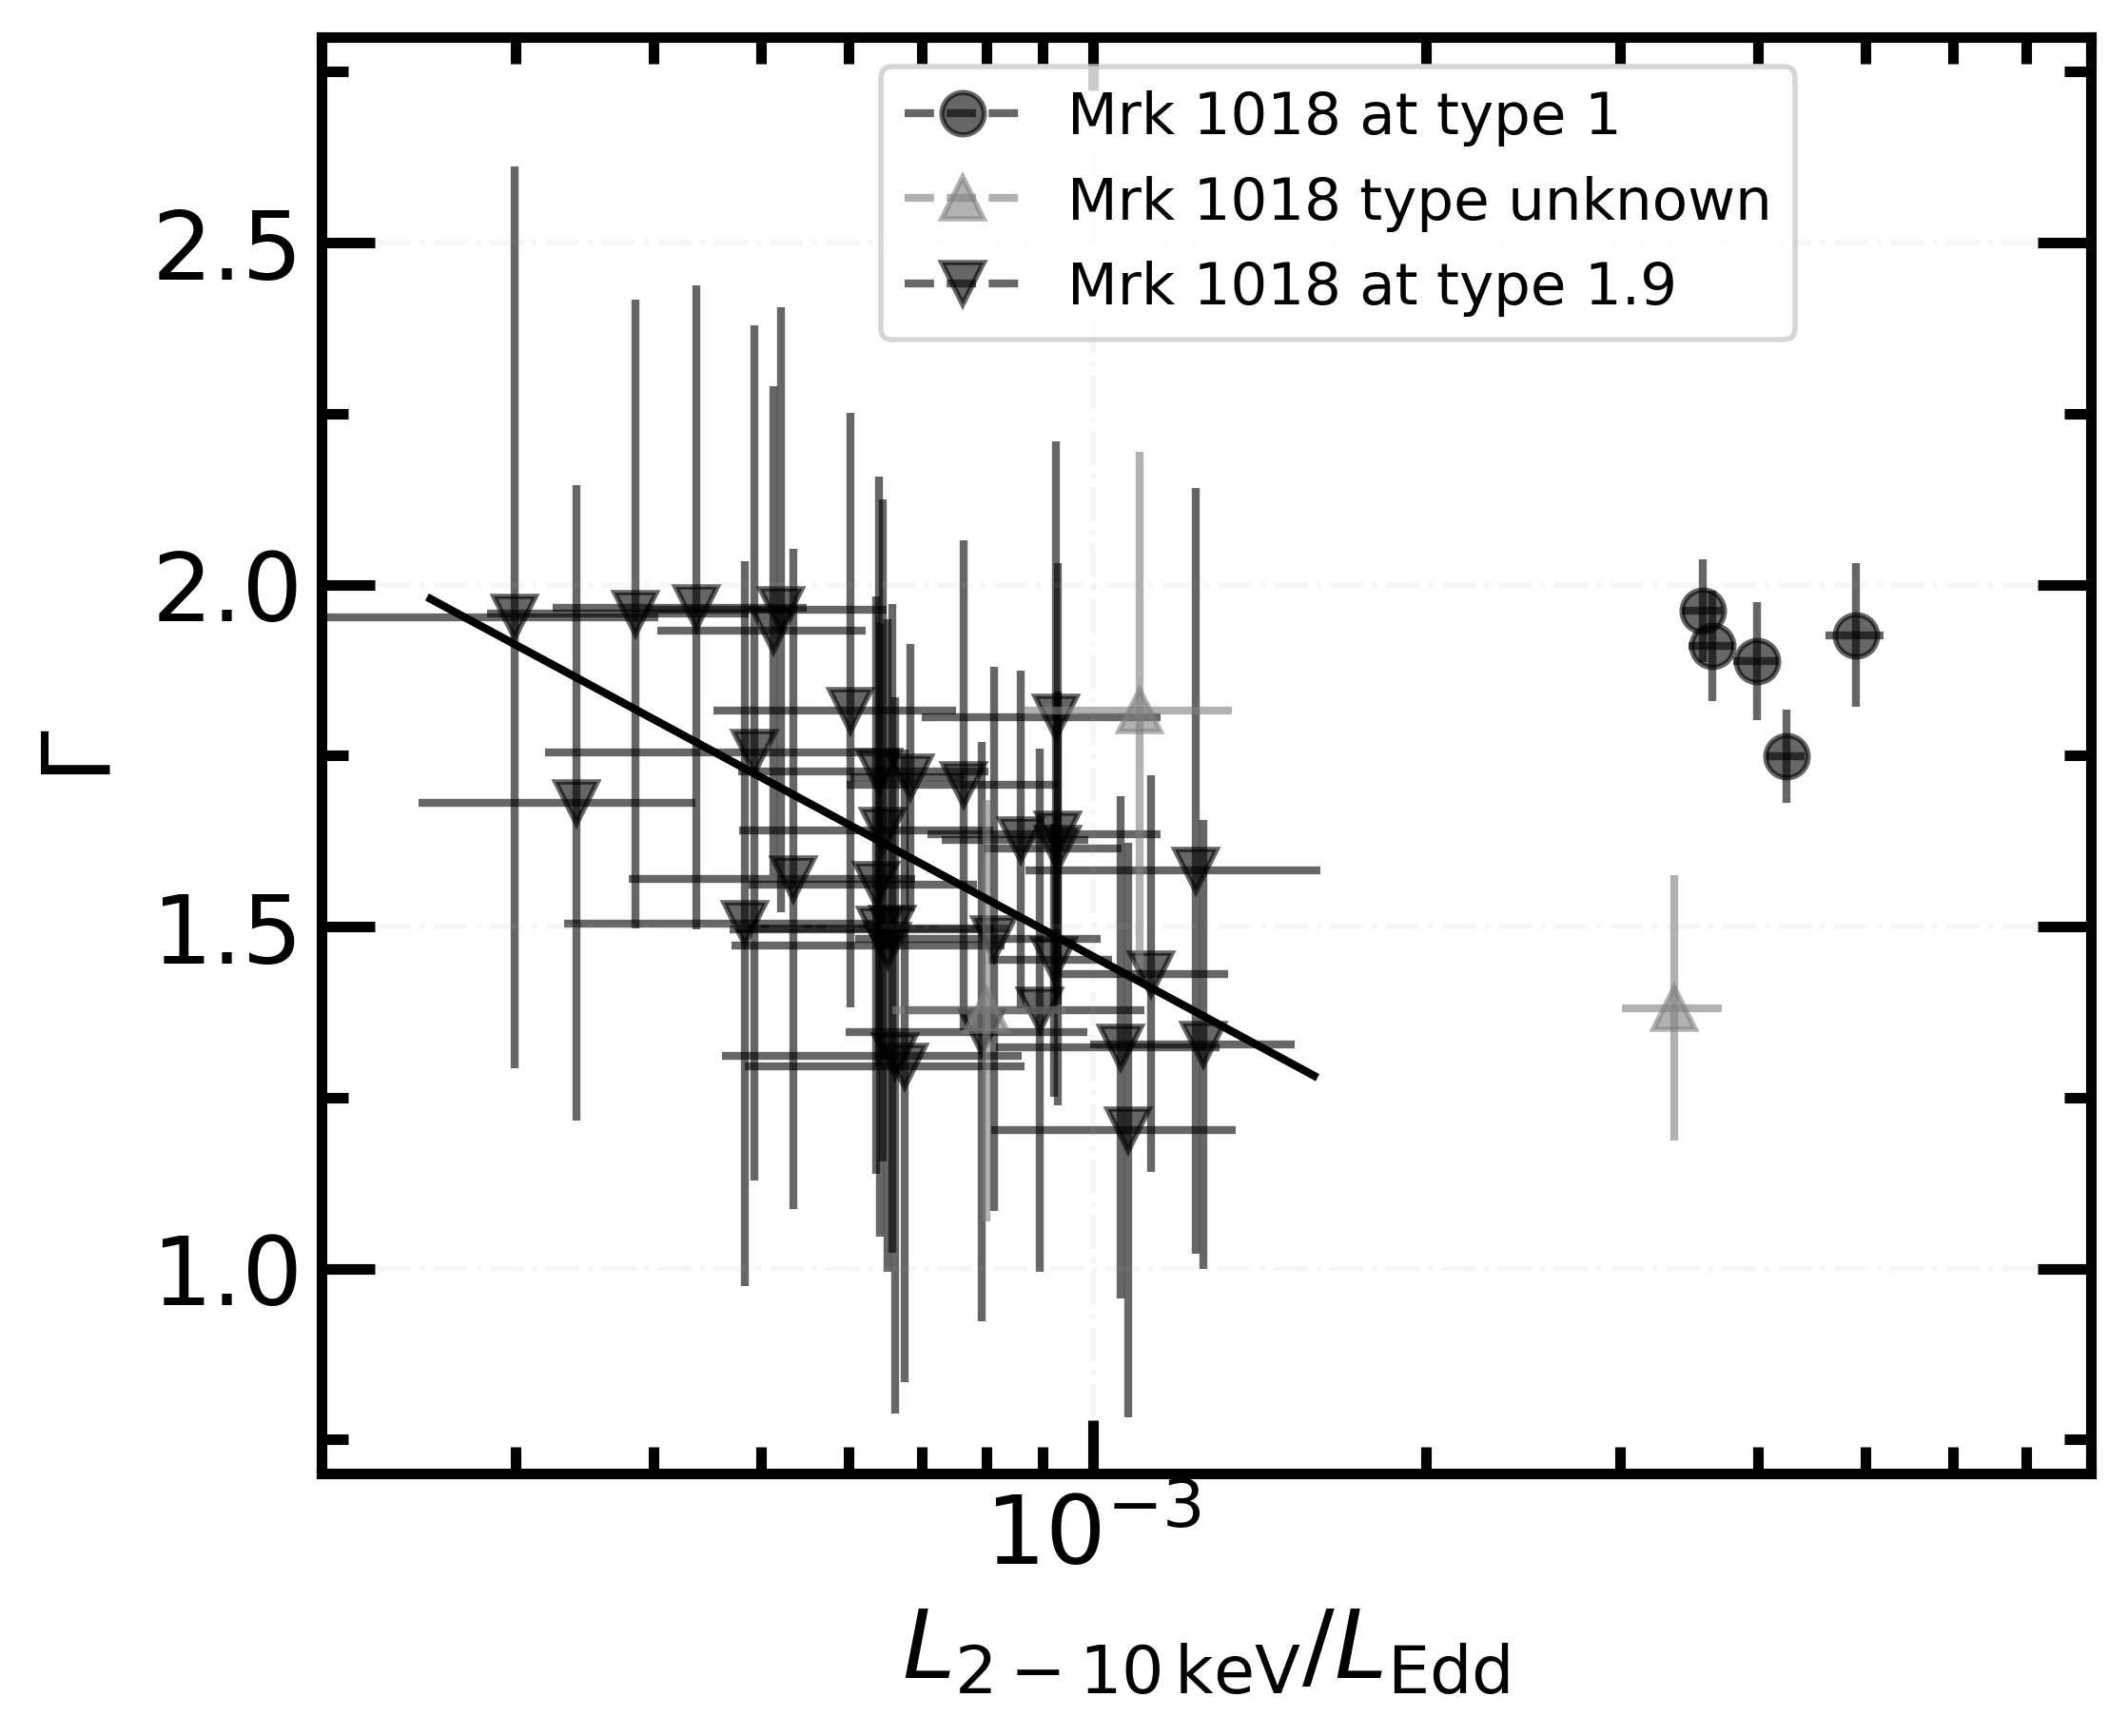
\includegraphics[width=\linewidth]{./pic/xrt_only-errorbar-Lrate-g-tmap_brokenlinear_dot.png}
    \caption{The $\Gamma$ - $L_\mathrm{X}/L_\mathrm{Edd}$ correlation. Only data of \xrt\, are included here. The dashed line represent the best fitting of the negative correlation in the type 1.9 phase.}
    \label{fig:xrayappendgood-Lrateandg-tmap}
\end{figure}
\begin{figure}
\centering
	% To include a figure from a file named example.*
	% Allowable file formats are eps or ps if compiling using latex
	% or pdf, png, jpg if compiling using pdflatex
	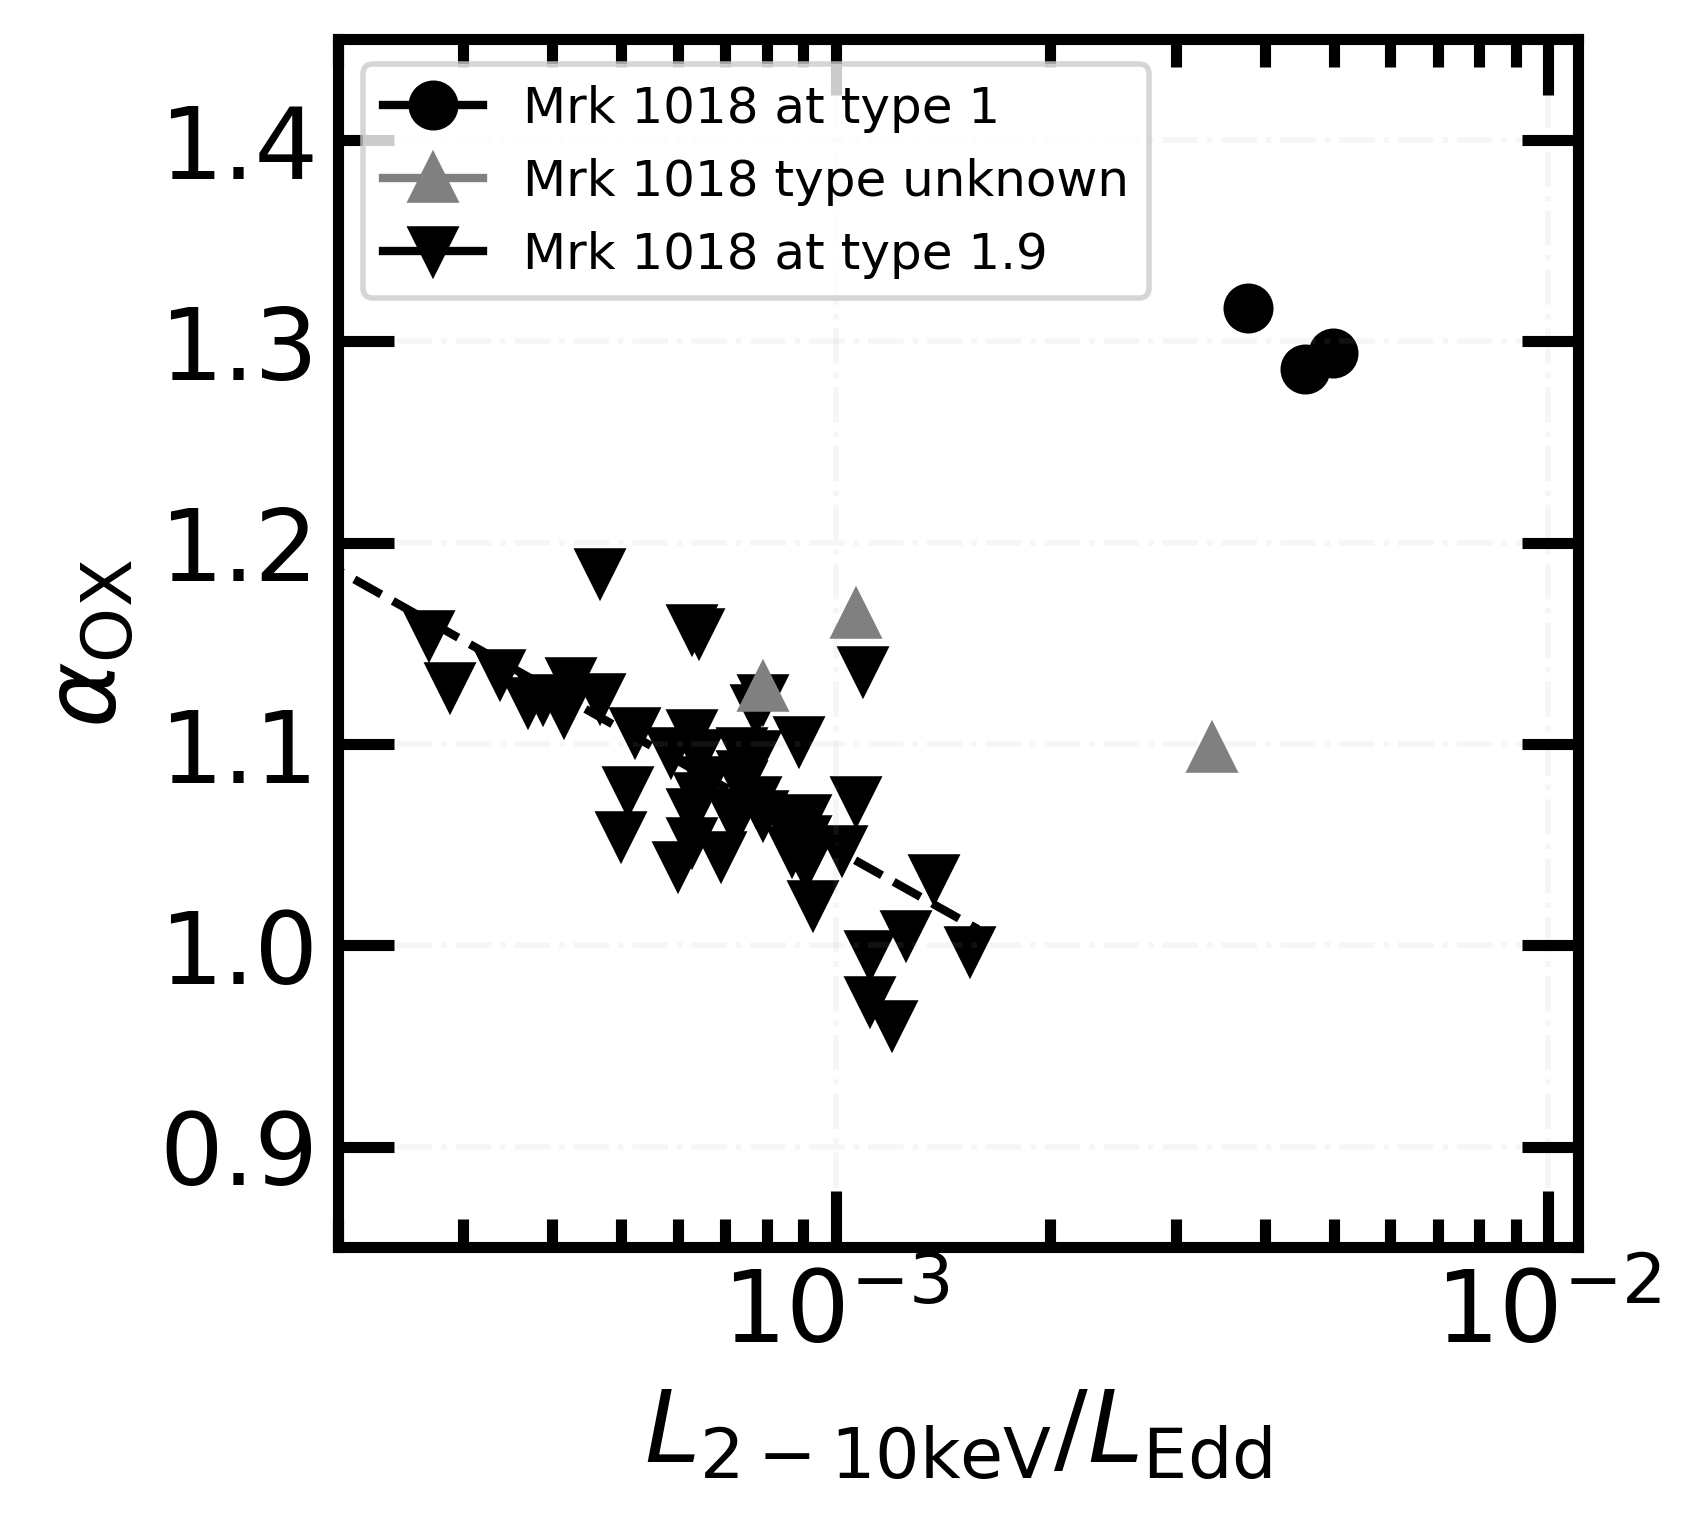
\includegraphics[width=\linewidth]{./pic/Mrk1018_2individuals_alpha_ox_L2-10.png}
    \caption{The $\alpha_\mathrm{OX}-L_{\mathrm{X}}/L_\mathrm{Edd}$ correlation. The dashed line represent the best fitting of the negative correlation in the type 1.9 phase.}   
    \label{fig:alpha_ox_lx}
\end{figure}


\subsection{Radio--X-ray luminosity correlation}
The correlation of the 5 GHz radio luminosity ($\log L_\mathrm{R}$) and 2--10~keV X-ray luminosity ($\log L_\mathrm{X}$) is presented in \autoref{fig:radio-xray-mass_relation_Plotkin2012}, where the quasi-simultaneous radio and X-ray observations within 100 days are adopted. The radio and X--ray luminosity follow a quite flat correlation during the luminosity range of $L_\mathrm{X}/L_\mathrm{Edd}$ $\sim$ 5$\times 10^{-4}$-- 4$\times 10^{-3}$, where the Spearman correlation coefficient is $0.2$ ($p=0.75$). Coincidently, the two points in 2017 and average of the $\log L_\mathrm{R}$ and $\log L_\mathrm{X}$ correlation of Mrk 1018 roughly follows the fundamental plane defined by the sample of AGN and XRB \citep[e.g.][]{2012MNRAS.419..267P}. But the points before 2016 deviate the fundamental plane where $L_\mathrm{R}\propto L_\mathrm{X}^{0.6}$.




\begin{figure}
\centering
	% To include a figure from a file named example.*
	% Allowable file formats are eps or ps if compiling using latex
	% or pdf, png, jpg if compiling using pdflatex
	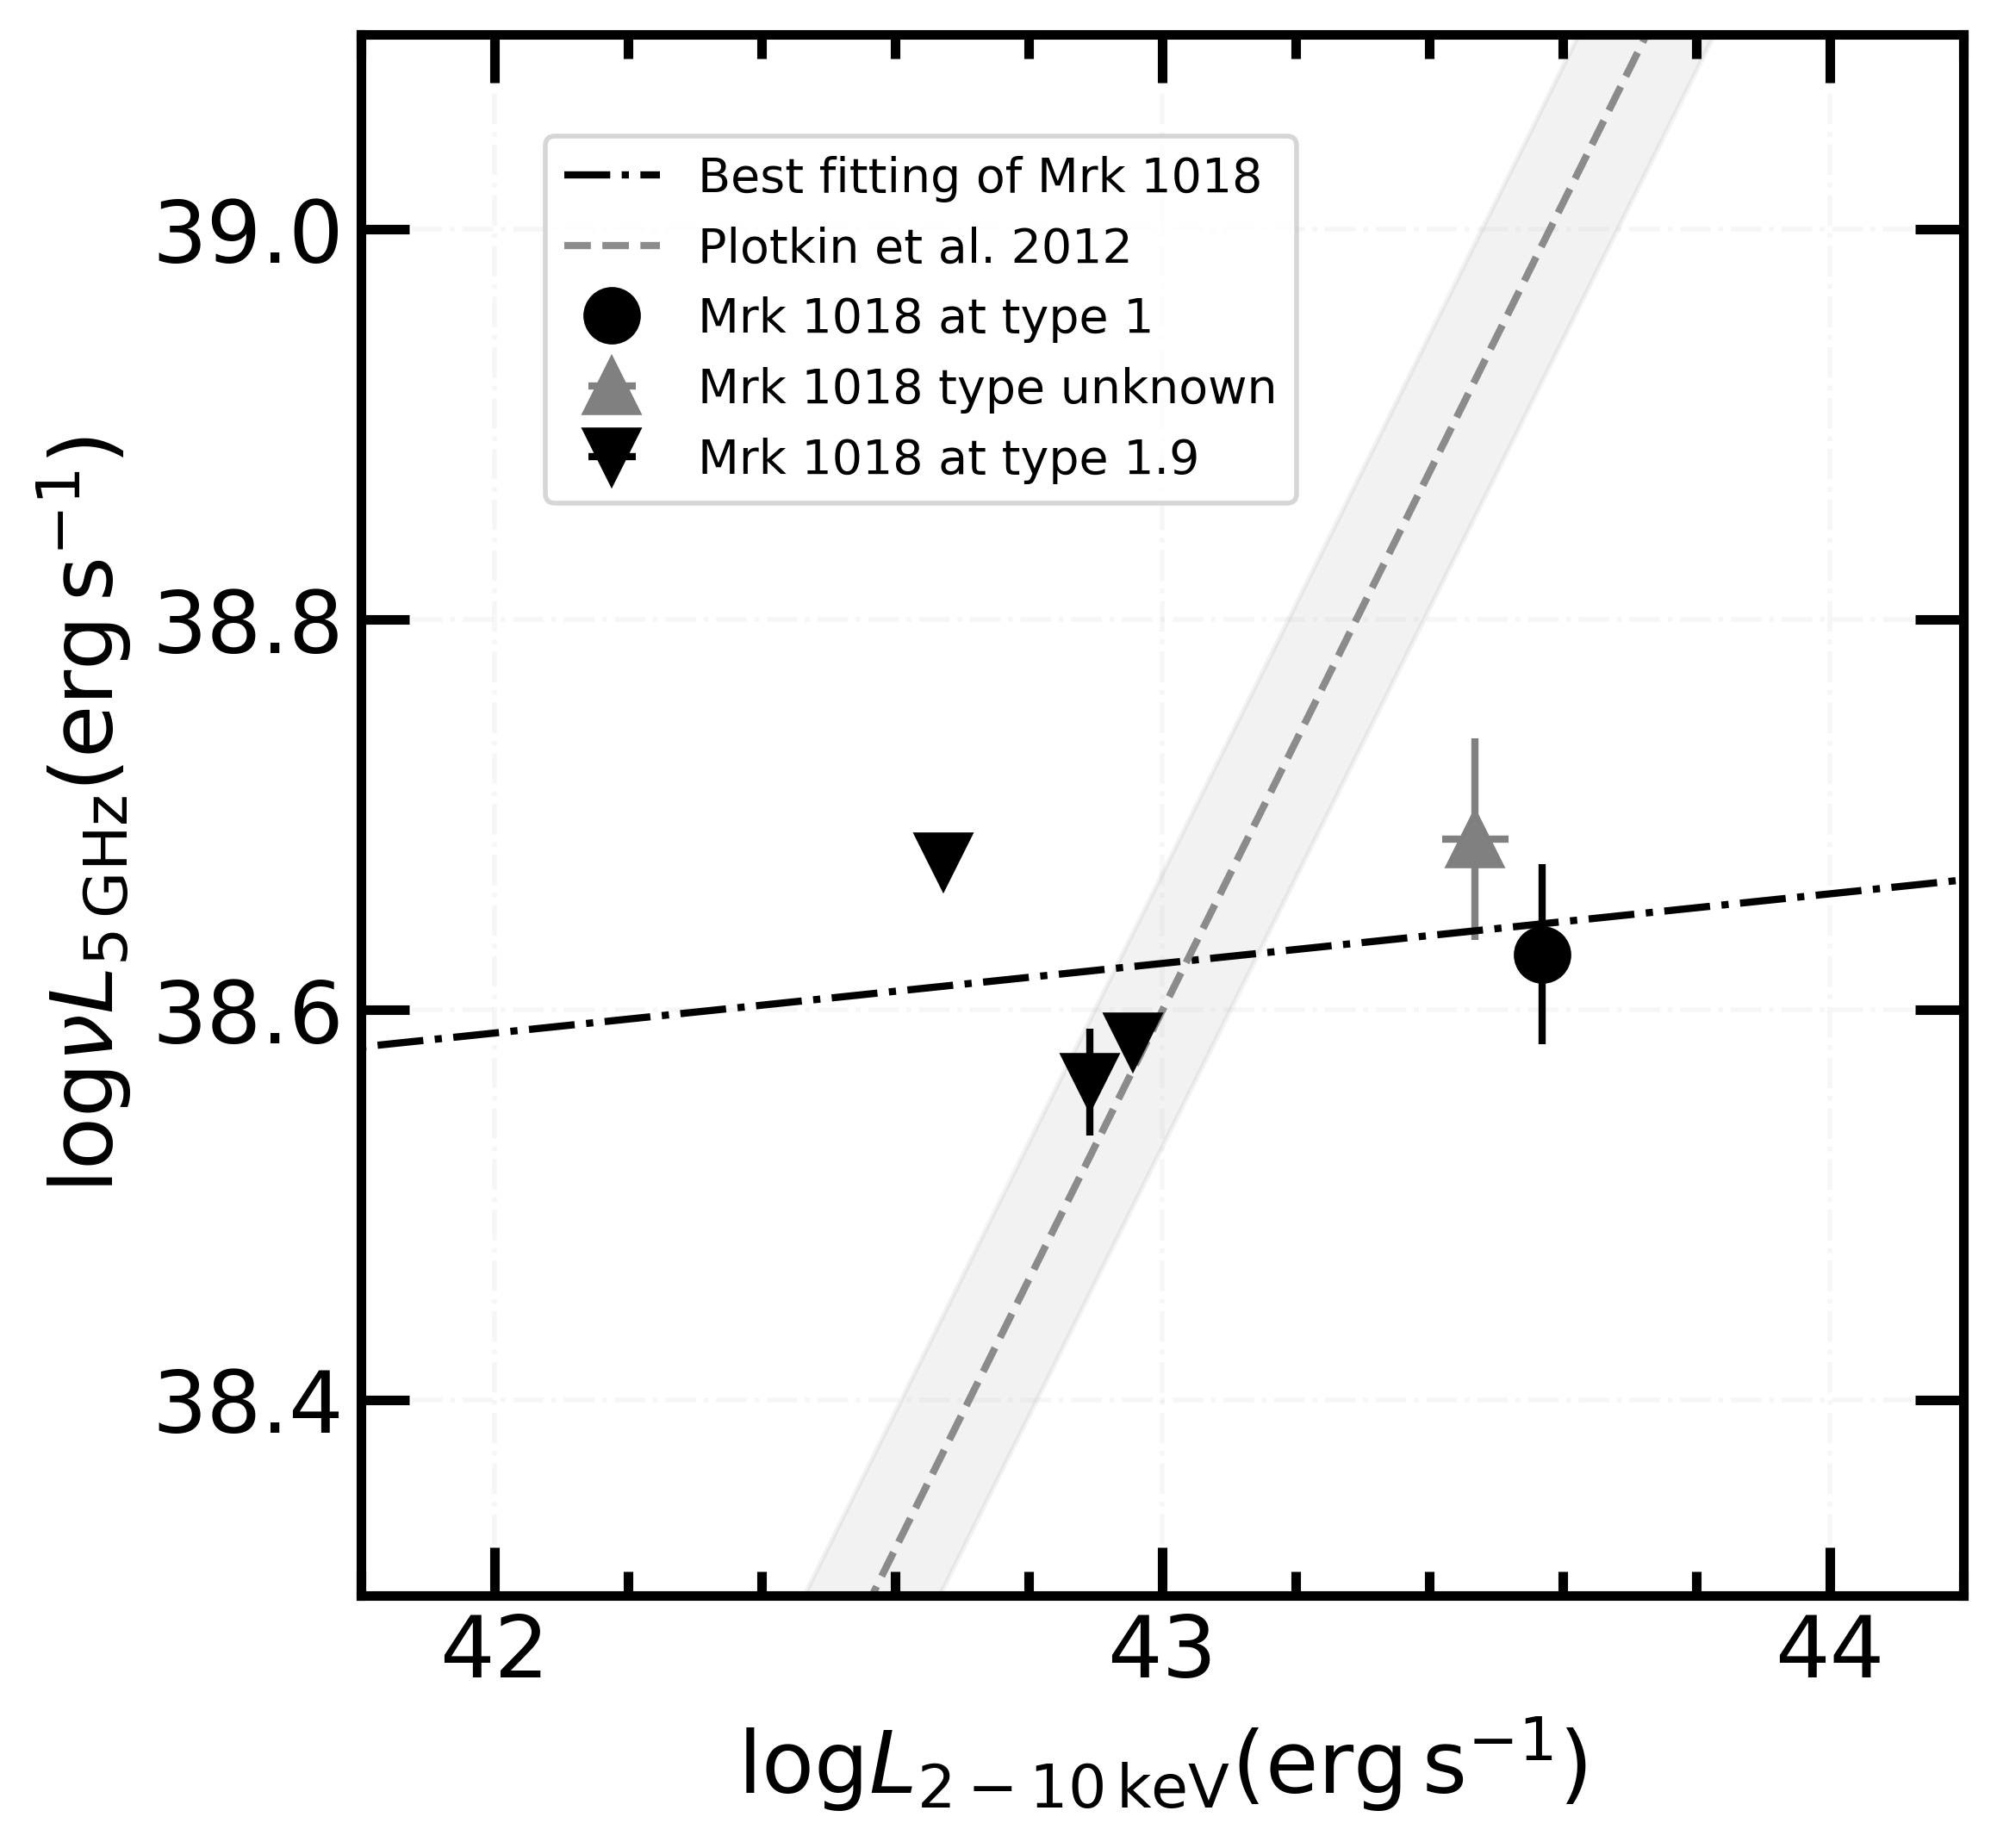
\includegraphics[width=\linewidth]{./pic/Mrk1018_radio_xray_Plotkin2012_Lx_near.png}
    \caption{The $\log L_\mathrm{R}$-$\log L_\mathrm{X}$ correlation. The dash-dot line represents the best-fitting line of Mrk~1018 with a slope of $\sim 0.04$. %The cross point represents the mean value of the radio and X-ray luminosity with the standard deviation as uncertainty. 
    The fundamental plane of a sample of black holes in \citet{2012MNRAS.419..267P} with a slope of $\sim 0.6$ is presented in the grey dashed line with intrinsic $\sigma=0.07$ for comparison.} 
    \label{fig:radio-xray-mass_relation_Plotkin2012}
\end{figure}
\section{Discussion}\label{sec:discussion}
\subsection{The spectral evolution and possible accretion mode transition }
\label{sec:spectral evolution}
\textcolor{red}{The hot accretion flow such as the Accretion Dominated Accretion Flow (ADAF) is thought to dominate the broad band emission from optical to X-ray \citep[see reviews in ][]{2014ARA&A..52..529Y} in low-luminosity AGNs (LLAGNs), while the optical/UV emission originates from the Shakura–Sunyaev disk \citep[SSD; e.g. ][]{2013ApJ...764....2Q} in luminous AGNs. The X-ray emission of AGNs is mainly comes from the Compton scattering in the hot ADAF or corona that stay below/above the cold SSD \citep[e.g.][]{1991ApJ...380L..51H}. The X-ray photon index reflect the properties of the hot corona, which is controlled by the electron temperature and optical depth of hot plasma(ADAF or corona).} The negative/positive correlation of $\Gamma$-$\log{L_\mathrm{X}/L_\mathrm{Edd}}$ below/above a critical value ($L_\mathrm{X}/L_\mathrm{Edd} \sim 10^{-3}$) has been found in both AGNs and BH XRBs samples \citep[e.g.][]{2008ApJ...682..212W,2009MNRAS.399..349G,2011A&A...530A.149Y,2015MNRAS.447.1692Y}. There is an evident anti-correlation of $\Gamma$-$\log{L_\mathrm{X}/L_\mathrm{Edd}}$ in the type 1.9 phase of Mrk~1018, which is similar to the low-luminosity AGNs and the low/hard state XRBs. The data in type 1 phase deviate the anti-correlation evidently. They may belong to the positive branch where the observational data are still limited. Mrk~1018 shares almost the same value of $L_\mathrm{X}/L_\mathrm{Edd}\sim 10^{-3}$ as the pivoting line of the negative/positive correlations of $\Gamma$-$\log{L_\mathrm{X}/L_\mathrm{Edd}}$ with the AGNs and the XRBs samples. The negative and positive correlations were attributed to ADAF and SSD-corona models, respectively. 






A flare was found during the decay phase, where the physical reason is still unclear. 


\textcolor{red}{During the re-flare, the spectrum becomes very hard ($\Gamma \sim 1.4$) as the X-ray luminosity increases, which could be explained by the increase of seed photons for comptonization causes the increase of optical depth. Our results suggests the type 1.9 is associated with the ADAF and the type 1 is associated with the SSD. The disappearance of the inner disk might be the explanation for the changing look.} The change of accretion mode is also suggested in other CL-AGNs \citep{2020ApJ...890L..29A} and highly variable AGN \citep{2020MNRAS.492.2335L}.  

The negative and positive correlations of \alphaox-$\log{L_\mathrm{X}/L_\mathrm{Edd}}$ have also been found in the low-luminosity AGNs\citep[e.g.][]{2011ApJ...739...64X,2017MNRAS.471.2848L} and luminous AGNs samples \citep[e.g.][]{2010A&A...512A..34L, 2013A&A...550A..71V,2016ApJ...819..154L}. \citet{2011MNRAS.413.2259S} simulated the spectral states of AGNs by analogy with BHXRBs, and found that the simulated AGNs at different spectral states and luminosity roughly follow a V-shape \alphaox--$L_\mathrm{bol}$ correlation (negetive/positive correlation below/above an critical value) \citep[see also in ][]{2019ApJ...883...76R}. \citet{2019arXiv190904676R} finds two CL-AGNs roughly follow a V-shape \alphaox--$L_\mathrm{UV}$ correlation when the two CL-AGNs are type 2 and type 1, respectively. \textcolor{red}{The ADAF model} can roughly explain the negative \alphaox\,--$L_\mathrm{bol}$ correlation at the lower luminosity branch \citep{2011ApJ...739...64X,2017MNRAS.471.2848L}, and the disk-corona model can explain the positive \alphaox\,--$L_\mathrm{bol}$ correlation at the higher luminosity branch \citep{2017A&A...602A..79L, 2018MNRAS.480.1247K,2019A&A...628A.135A}. There is an evident anti-correlation of \alphaox-$\log{L_\mathrm{X}/L_\mathrm{Edd}}$ in the type 1.9 AGN phase of Mrk~1018, which is similar to the low-luminosity AGNs. The pivoting line of the negative/positive correlations of \alphaox-$\log{L_\mathrm{bol}/L_\mathrm{Edd}}$ is roughly at $L_\mathrm{bol}/L_\mathrm{Edd} \sim$ $10^{-3}$, assuming that $L_\mathrm{bol}/L_\mathrm{X} \sim$ $30$ \citep[see][]{2011ApJ...739...64X,2017MNRAS.471.2848L}.  The anti-correlation of \alphaox-$\log{L_\mathrm{X}/L_\mathrm{Edd}}$ in the type 1.9 and the evident deviation in the type 1 also supports the accretion mode is different in the type 1 and type 1.9 AGN phase for Mrk~1018.     

The physical reason for triggering the changing-look is still unclear. Some models of the broad line region (BLR) \citep[see a recent review in ][and references therein]{2019OAst...28..200C} related with the SSD can be account for the type change in the CL-AGNs. For example, in the disk-wind model for the BLR origin, the AGNs evolve from type 1 to type 1.9 as the luminosity decreases \citep[see][]{2014MNRAS.438.3340E}. \citet{2018MNRAS.480.3898N} suggests that the soft X-ray excess contributes most ionizing photons, and the drop of soft X-ray excess causes the disappearance of broad emission line \citep[see also in ][]{2020MNRAS.492.2335L}. \textcolor{red}{ It has been observed that the broad line luminosity is positively correlated with the UV luminosity, and the broad line width is negatively correlated with the UV luminosity \citep[e.g.][]{2019ApJ...885...44D}. When the UV luminosity decreases, the broad line emission would decrease and the line width would broaden to be difficult to detect. We did detect the decay in both the X-ray and UV bands during the changing-look.} If there is a critical luminosity and it is below the peak of the re-flare, then Mrk~1018 would change its type back and forth between type 1 and type 1.9 during the re-flare. The UV luminosity only varied by a factor of $\sim$1.4 and the X-ray luminosity varied by a factor of $\sim$3.2 at the peak of the re-flare. If the critical luminosity is above the peak of re-flare, then the changing-look would happen in earlier timeline before 2013 and the changing-look would be more likely associated with the decline of UV luminosity since the peak X-ray luminosity of the re-flare is close to the X-ray luminosity in type 1. The optical confirmation would help to find out which one directly influence the type change.



\subsection{The variability timescale}
\label{sec:timescale}
The flux variations of AGNs on different timescales and different wavelengths have been studied for a long time \citep[see reviews in ][]{1997ARA&A..35..445U}. We calculate the \textit{e}-folding decay timescale is $\sim$ 1000 days  during the rapid decay in both the X-ray and UV bands, which is consistent with the changing-look timescale of less than 5 years (between 2010 Nov. and 2015 Jan.). The viscous timescale at typical outer disk radius of $R_\mathrm{disk}$ around hundreds of $R_g$ is much longer than the changing-look timescale \citep[see also][]{2012MmSAI..83..469L,2018MNRAS.475.1190Y}. \textcolor{red}{The changing-look timescale might correspond the timescale of the evaporation of the inner disk \citep{}.} The thermal timescale is considered as the origin of the short-term (tens of days) variability in CL-AGNs. The rise timescale $\sim$ 98 days of the re-flare is consistent with the thermal timescale assuming R $\sim$ 200 $R_g$. Turn-on for CL-AGN could happen within timescale as short as $\sim$70 days\citep[e.g.][]{2019MNRAS.487.4057K}, which is suggested to be mostly compatible with the thermal timescale of $\sim$ 99 days assuming an optical emission distance of R $\sim$ 400 $R_g$. But we cannot draw a conclusion that the type change happened during the re-flare within such short timescale for Mrk~1018.


\subsection{R-X correlation}
It is widely accepted that there is a non-linear correlation between the 5 GHz radio luminosity and the 2--10 keV X-ray luminosity spanning over different mass black holes from the super-massive black holes to stellar mass black holes. The $L_\mathrm{R}$ is proportional to $L_\mathrm{X}^{0.6}$ \citep{2003MNRAS.345.1057M,2004A&A...414..895F}. However, there are some sources following a steeper R-X correlation with a power-law index of $\sim$1.4 at the high $L_\mathrm{X}$, a flat R-X correlation with a power-law index of $\sim$0 at the moderate $L_\mathrm{X}$, and the standard R-X correlation with a powerlaw index $\sim$0.6 at low luminosity \citep[e.g.][]{2011MNRAS.414..677C,2014ApJ...788...52C,2016MNRAS.463.2287X}. The physical reason of this ``hybrid" R-X correlation is still under debate. The slope change of the correlation may attribute to the different accretion modes or jet physics at low and high luminosity\citep{2016MNRAS.456.4377X,2018MNRAS.481.4513I,2018MNRAS.473.4122E}. The flat R-X correlation of Mrk~1018 is much shallower than the correlation of a sample of black holes in \citet{2012MNRAS.419..267P}. \textcolor{red}{It implies that the radio variability timescale is much longer than X-ray or Mrk~1018 is accreting in the different mode from the samples. }



\section{Summary}
\label{sec:conclusion}
The main results are summarized as follows,
\begin{enumerate}

\item We present the long-term and multi-wavelength variabilities for the CL-AGN of Mrk 1018. We find that optical/UV emission start to decline in type I case even the X-ray emission is roughly unchanged before a rapid decay to type 1.9 during 2010-2015. We also find a re-flare in both optical and X-ray bands during the decay.   

\item The negative correlations of $\Gamma$-$L_\mathrm{X}/L_\mathrm{Edd}$ and \alphaox-$L_\mathrm{X}/L_\mathrm{Edd}$ in type 1.9 are consisted with the prediction of the radiatively inefficient accretion phase (e.g., ADAF). The Type I case evidently deviate from the negative correlations even the data are still limited, which may stay in a radiatively efficient SSD/corona phase. Therefore, the change of broad emission lines is most possibly regulated by underlying accretion mode. 

\item The radio emission in CL-AGN of Mrk~1018 is roughly unchanged during the changing look, even it is slightly declined about $\sim$ 20\% from 2015 to 2017. Therefore, radio--X-ray correlation is quite flat in Mrk 1018, which is much shallower than that found in low-luminosity AGNs and low-hard state XRBs with a slope of $\sim 0.6$. 

\end{enumerate}
 Further simultaneous observations in multi-wavelength bands are required to understand the evolution of AGN types with spectra and luminosity. 
 



\section*{Acknowledgements}
We thank the anonymous referee for useful comments and suggestions. We thank Prof Minfeng Gu for the discussions on the radio observations of CL-AGNs and Dr Linhui Wu and Minhua Zhou for discussions on the VLA data reduction. B.L. and Q.W. are supported in part by the NSFC (grant U1931203); Z.Y. is supported in part by the Natural Science Foundation of China (grants 11773055, U1938114), the Youth Innovation Promotion Association of CAS (ids. 2020265); W.Y. would like to acknowledge the support in part by the National Program on Key Research and Development Project (Grant No.2016YFA0400804) and the National Natural Science Foundation of China (grant number 11333005 and U1838203).

%Chris Done for her friendly help with the usage of host galaxy model
%%%%%%%%%%%%%%%%%%%%%%%%%%%%%%%%%%%%%%%%%%%%%%%%%%

\section*{Data Availability}
The data underlying this article are available through HEASARC Browse database and NRAO Science Data Archive.
%%%%%%%%%%%%%%%%%%%%%%%%%%%%%%%%%%%%%%%%%%%%%%%%%%

%%%%%%%%%%%%%%%%%%%% REFERENCES %%%%%%%%%%%%%%%%%%

% The best way to enter references is to use BibTeX:

\bibliographystyle{mnras}
\bibliography{refMrk1018all.bib} % if your bibtex file is called example.bib
%\clearpage

% Alternatively you could enter them by hand, like this:
% This method is tedious and prone to error if you have lots of references
%\begin{thebibliography}{99}
%\bibitem[\protect\citeauthoryear{Author}{2012}]{Author2012}Author A.~N., 2013, Journal of Improbable Astronomy, 1, 1
%\bibitem[\protect\citeauthoryear{Others}{2013}]{Others2013}Others S., 2012, Journal of Interesting Stuff, 17, 198
%\end{thebibliography}

%%%%%%%%%%%%%%%%%%%%%%%%%%%%%%%%%%%%%%%%%%%%%%%%%%
%%%%%%%%%%%%%%%%% APPENDICES %%%%%%%%%%%%%%%%%%%%%

%%%%%%%%%%%%%%%%%%%%%%%%%%%%%%%%%%%%%%%%%%%%%%%%%%

% Don't change these lines
\bsp	% typesetting comment
\label{lastpage}
%\clearpage
\appendix
\section{Appendix}
\begin{center}
%\centering
\footnotesize
\onecolumn
\begin{longtable}{cccccc}
\caption{{\bfseries X-ray data of Mrk~1018. } Columns include the date of observations, observation ID, the telescope, the photon index $\Gamma$ with 90\% uncertainty, and Galactic-absorption corrected 2--10~keV X-ray flux.
\label{tab:tablexray}} \\
\hline 
\hline
 Date   &   ObsID & Telescope   &  $\Gamma$ & $F_{\rm{2-10~keV}}$ &    \\ 
 (MJD)  &         &             &           & [$10^{-12}$ erg cm$^{-2}$\rm{s}$^{-1}$] &  \\ 
\hline
\endfirsthead
\multicolumn{5}{c}%
{{\bfseries \tablename\ \thetable{} -- continued from previous page}} \\
\hline 
\hline
 Date   &   ObsID & Telescope   &  $\Gamma$ & $F_{\rm{2-10~keV}}$ &    \\ 
 (MJD)  &         &             &           & [$10^{-12}$ erg cm$^{-2}$\rm{s}$^{-1}$] &  \\ 
\hline
\endhead
\hline 
\multicolumn{5}{c}{
The superscripts $^{(a)}$ and $^{(b)}$ represent the fitting results from \citet{2012ApJ...745..107W} and \citet{2016A&A...593L...9H}, repectively.}\\ \
\endfoot
\hline 
\multicolumn{5}{c}{Notes: The facility is represented by C-\chandra, S-\swift, X-\xmm, N-\nustar and Su-\suzaku.}\\ \
\endlastfoot

53385 & 201090201 & X & 1.68 $\pm$ 0.11 & 10.40 $\pm$ 0.50 & \\
53587 & 35166001 & S & 1.94 $\pm$ 0.06 & 11.75 $\pm$ 0.81 & \\
54273 & 30955002 & S & 1.91 $\pm$ 0.05 & 8.91 $\pm$ 0.62 & \\
54275 & 30955003 & S & 1.95 $\pm$ 0.04 & 8.91 $\pm$ 0.41 & \\
54628 & 35776001 & S & 1.73 $\pm$ 0.04 & 10.72 $\pm$ 0.49 & \\
54685 & 554920301 & X & 1.79 $\pm$ 0.03 & 11.50 $\pm$ 0.20 & \\
55015 & 704044010$^{a}$ & Su  & 2.00 $\pm$ 0.03 & 10.00 $\pm$ 0.50  \\
55527 & 12868$^{b}$ & C  & 1.68 $\pm$ 0.04 & 9.20 $\pm$ 0.20  \\
56352 & 49654001 & S & 1.82 $\pm$ 0.23 & 2.51 $\pm$ 0.75 & \\
56450 & 49654002 & S & 1.45 $\pm$ 0.09 & 7.94 $\pm$ 0.91 & \\
56817 & 49654004 & S & 1.39 $\pm$ 0.19 & 1.86 $\pm$ 0.39 & \\
57428 & 60160087002 & N & 1.85 $\pm$ 0.08 & 1.80 $\pm$ 0.10 & \\
57429 & 80898001 & S & 1.72 $\pm$ 0.12 & 1.62 $\pm$ 0.26 & \\
57434 & 80898002 & S & 1.46 $\pm$ 0.12 & 2.19 $\pm$ 0.35 & \\
57443 & 18789 & C & 1.68 $\pm$ 0.03 & 1.27 $\pm$ 0.03 & \\
57801 & 19560 & C & 1.61 $\pm$ 0.02 & 2.44 $\pm$ 0.02 & \\
58123 & 60301022002 & N & 1.80 $\pm$ 0.06 & 2.10 $\pm$ 0.10 & \\
58124 & 88207001 & S & 1.63 $\pm$ 0.15 & 2.04 $\pm$ 0.38 & \\
58126 & 20366 & C & 1.60 $\pm$ 0.03 & 1.79 $\pm$ 0.04 & \\
58173 & 88207002 & S & 1.60 $\pm$ 0.16 & 2.00 $\pm$ 0.41 & \\
58180 & 20367 & C & 1.63 $\pm$ 0.04 & 1.56 $\pm$ 0.03 & \\
58182 & 60301022003 & N & 1.80 $\pm$ 0.06 & 1.50 $\pm$ 0.07 & \\
58281 & 20368 & C & 1.64 $\pm$ 0.03 & 1.74 $\pm$ 0.04 & \\
58316 & 60301022005 & N & 1.74 $\pm$ 0.05 & 2.00 $\pm$ 0.09 & \\
58316 & 88207003 & S & 1.63 $\pm$ 0.14 & 2.19 $\pm$ 0.40 & \\
58362 & 35776002 & S & 1.98 $\pm$ 0.29 & 1.00 $\pm$ 0.37 & \\
58363 & 35776003 & S & 1.41 $\pm$ 0.29 & 1.74 $\pm$ 0.64 & \\
58364 & 35776004 & S & 1.34 $\pm$ 0.23 & 2.40 $\pm$ 0.66 & \\
58365 & 35776005 & S & 1.48 $\pm$ 0.23 & 1.82 $\pm$ 0.50 & \\
58368 & 35776006 & S & 1.44 $\pm$ 0.18 & 2.63 $\pm$ 0.61 & \\
58369 & 35776007 & S & 1.64 $\pm$ 0.19 & 2.63 $\pm$ 0.61 & \\
58370 & 20369 & C & 1.63 $\pm$ 0.03 & 2.65 $\pm$ 0.06 & \\
58370 & 35776008 & S & 1.81 $\pm$ 0.25 & 2.14 $\pm$ 0.69 & \\
58374 & 35776010 & S & 1.56 $\pm$ 0.34 & 1.86 $\pm$ 0.81 & \\
58375 & 35776011 & S & 1.39 $\pm$ 0.23 & 2.04 $\pm$ 0.56 & \\
58378 & 35776014 & S & 1.33 $\pm$ 0.21 & 2.95 $\pm$ 0.75 & \\
58384 & 35776015 & S & 1.60 $\pm$ 0.35 & 2.82 $\pm$ 1.30 & \\
58385 & 35776016 & S & 1.16 $\pm$ 0.21 & 3.63 $\pm$ 0.92 & \\
58390 & 35776017 & S & 1.49 $\pm$ 0.24 & 1.86 $\pm$ 0.56 & \\
58390 & 35776018 & S & 1.72 $\pm$ 0.22 & 1.74 $\pm$ 0.48 & \\
58391 & 35776019 & S & 1.51 $\pm$ 0.29 & 1.51 $\pm$ 0.52 & \\
58392 & 35776020 & S & 1.50 $\pm$ 0.27 & 1.48 $\pm$ 0.51 & \\
58393 & 35776021 & S & 1.13 $\pm$ 0.26 & 2.57 $\pm$ 0.77 & \\
58395 & 35776023 & S & 1.74 $\pm$ 0.27 & 1.48 $\pm$ 0.51 & \\
58396 & 35776024 & S & 1.82 $\pm$ 0.27 & 1.38 $\pm$ 0.48 & \\
58399 & 35776026 & S & 1.64 $\pm$ 0.24 & 2.14 $\pm$ 0.64 & \\
58399 & 35776027 & S & 1.97 $\pm$ 0.27 & 1.20 $\pm$ 0.42 & \\
58402 & 35776029 & S & 1.74 $\pm$ 0.27 & 1.70 $\pm$ 0.63 & \\
58409 & 35776032 & S & 1.02 $\pm$ 0.29 & 2.09 $\pm$ 0.72 & \\
58410 & 35776033 & S & 1.98 $\pm$ 0.28 & 0.87 $\pm$ 0.32 & \\
58412 & 35776034 & S & 1.01 $\pm$ 0.24 & 3.24 $\pm$ 0.89 & \\
58413 & 35776035 & S & 1.36 $\pm$ 0.26 & 1.82 $\pm$ 0.59 & \\
58417 & 35776036 & S & 1.12 $\pm$ 0.27 & 2.14 $\pm$ 0.69 & \\
58418 & 35776037 & S & 2.03 $\pm$ 0.42 & 0.63 $\pm$ 0.31 & \\
58420 & 35776038 & S & 1.72 $\pm$ 0.44 & 0.91 $\pm$ 0.50 & \\
58420 & 35776039 & S & 1.33 $\pm$ 0.32 & 1.51 $\pm$ 0.56 & \\
58422 & 35776040 & S & 1.30 $\pm$ 0.28 & 1.55 $\pm$ 0.53 & \\
58423 & 35776041 & S & 1.55 $\pm$ 0.32 & 1.41 $\pm$ 0.59 & \\
58424 & 35776042 & S & 1.94 $\pm$ 0.22 & 1.17 $\pm$ 0.35 & \\
58425 & 35776043 & S & 1.78 $\pm$ 0.31 & 0.98 $\pm$ 0.38 & \\
58426 & 35776044 & S & 1.15 $\pm$ 0.35 & 2.00 $\pm$ 0.87 & \\
58427 & 35776045 & S & 1.51 $\pm$ 0.33 & 1.10 $\pm$ 0.45 & \\
58428 & 35776046 & S & 1.48 $\pm$ 0.29 & 1.51 $\pm$ 0.52 & \\
58429 & 35776047 & S & 1.38 $\pm$ 0.30 & 1.74 $\pm$ 0.60 & \\
58430 & 20370 & C & 1.64 $\pm$ 0.04 & 1.39 $\pm$ 0.03 & \\
58433 & 35776049 & S & 1.76 $\pm$ 0.38 & 1.10 $\pm$ 0.50 & \\
58434 & 35776050 & S & 1.56 $\pm$ 0.30 & 1.23 $\pm$ 0.45 & \\
58436 & 35776051 & S & 1.57 $\pm$ 0.26 & 1.48 $\pm$ 0.48 & \\
58437 & 35776052 & S & 1.17 $\pm$ 0.30 & 1.82 $\pm$ 0.63 & \\
58439 & 35776054 & S & 1.65 $\pm$ 0.29 & 1.48 $\pm$ 0.51 & \\
58444 & 35776056 & S & 1.21 $\pm$ 0.25 & 2.51 $\pm$ 0.75 & \\
58445 & 35776057 & S & 1.99 $\pm$ 0.42 & 0.68 $\pm$ 0.34 & \\
58446 & 35776058 & S & 1.27 $\pm$ 0.43 & 1.70 $\pm$ 0.98 & \\
58520 & 21432 & C & 1.66 $\pm$ 0.03 & 1.71 $\pm$ 0.03 & \\
58521 & 22082 & C & 1.65 $\pm$ 0.03 & 1.87 $\pm$ 0.04 & \\
58663 & 35776059 & S & 1.69 $\pm$ 0.28 & 0.79 $\pm$ 0.27 & \\
\hline

\end{longtable}

\end{center}
%55015 & 704044010$^{a}$ & Su  & 2.00 $\pm$ 0.03 & 10.00 $\pm$ 0.50  \\
%55527 & 12868$^{b}$ & C  & 1.68 $\pm$ 0.04 & 9.20 $\pm$ 0.20  \\



%len(uvot_uuu),len(uvot_uw1),len(uvot_um2),len(uvot_uw2)
\begin{center}
\centering
%\centerline{Table 1: the basic parameters of CL-AGN sample.}
%\end{center}
\footnotesize
\onecolumn
\begin{longtable}{ccccccccc}
\caption{{ \bf UVOT data of Mrk~1018. } Columns include the date of observations and the absorption and host corrected flux. 
\label{tab:tableuvot}} \\
\hline
\hline
Date   &  U     & Date     &  UVW1  &  Date  &  UVM2   &  Date  &   UVW2 &   \\ 
(MJD)  &  [mJy] &  (MJD)   &[mJy]   & (MJD)  & [mJy]   & (MJD)  & [mJy]  & \\ 
\hline
\endfirsthead
\multicolumn{8}{c}%
{{\bfseries \tablename\ \thetable{} -- continued from previous page}} \\
\hline 
\hline
Date   &  U     & Date     &  UVW1  &  Date  &  UVM2   &  Date  & UVW2   &   \\ 
(MJD)  &  [mJy] &  (MJD)   &[mJy]   & (MJD)  & [mJy]   & (MJD)  & [mJy]  & \\ \\ \hline 
\endhead
53587 & 3.77 $\pm$ 0.10 & 53587 & 3.56 $\pm$ 0.11 & 53587 & 3.51 $\pm$ 0.06 & 53587 & 3.53 $\pm$ 0.08 & \\
54628 & 2.86 $\pm$ 0.08 & 54271 & 2.99 $\pm$ 0.09 & 54628 & 2.46 $\pm$ 0.04 & 54273 & 2.92 $\pm$ 0.06 & \\
56352 & 0.35 $\pm$ 0.04 & 54275 & 3.12 $\pm$ 0.09 & 56352 & 0.34 $\pm$ 0.02 & 54628 & 2.35 $\pm$ 0.05 & \\
56450 & 0.47 $\pm$ 0.03 & 54628 & 2.60 $\pm$ 0.08 & 56450 & 0.41 $\pm$ 0.02 & 56352 & 0.24 $\pm$ 0.01 & \\
56817 & 0.08 $\pm$ 0.02 & 56352 & 0.32 $\pm$ 0.02 & 56817 & 0.09 $\pm$ 0.01 & 56450 & 0.39 $\pm$ 0.01 & \\
57429 & 0.12 $\pm$ 0.02 & 56450 & 0.48 $\pm$ 0.02 & 57429 & 0.07 $\pm$ 0.01 & 56817 & 0.09 $\pm$ 0.01 & \\
57434 & 0.05 $\pm$ 0.02 & 56817 & 0.13 $\pm$ 0.01 & 57434 & 0.06 $\pm$ 0.00 & 57429 & 0.06 $\pm$ 0.00 & \\
58124 & 0.07 $\pm$ 0.01 & 57429 & 0.09 $\pm$ 0.01 & 58362 & 0.07 $\pm$ 0.01 & 57434 & 0.06 $\pm$ 0.01 & \\
58316 & 0.07 $\pm$ 0.01 & 57434 & 0.08 $\pm$ 0.01 & 58363 & 0.06 $\pm$ 0.01 & 58173 & 0.08 $\pm$ 0.00 & \\
58362 & 0.12 $\pm$ 0.03 & 58362 & 0.12 $\pm$ 0.02 & 58364 & 0.07 $\pm$ 0.01 & 58362 & 0.08 $\pm$ 0.01 & \\
58363 & 0.05 $\pm$ 0.02 & 58363 & 0.09 $\pm$ 0.01 & 58365 & 0.08 $\pm$ 0.01 & 58363 & 0.08 $\pm$ 0.01 & \\
58364 & 0.09 $\pm$ 0.03 & 58364 & 0.10 $\pm$ 0.01 & 58368 & 0.06 $\pm$ 0.01 & 58364 & 0.07 $\pm$ 0.01 & \\
58365 & 0.03 $\pm$ 0.02 & 58365 & 0.10 $\pm$ 0.01 & 58369 & 0.05 $\pm$ 0.01 & 58365 & 0.08 $\pm$ 0.01 & \\
58368 & 0.07 $\pm$ 0.02 & 58368 & 0.08 $\pm$ 0.01 & 58370 & 0.06 $\pm$ 0.01 & 58368 & 0.07 $\pm$ 0.01 & \\
58369 & 0.06 $\pm$ 0.02 & 58369 & 0.09 $\pm$ 0.01 & 58374 & 0.06 $\pm$ 0.01 & 58369 & 0.05 $\pm$ 0.01 & \\
58370 & 0.05 $\pm$ 0.03 & 58370 & 0.13 $\pm$ 0.02 & 58375 & 0.05 $\pm$ 0.01 & 58370 & 0.08 $\pm$ 0.01 & \\
58374 & 0.09 $\pm$ 0.03 & 58374 & 0.10 $\pm$ 0.01 & 58375 & 0.06 $\pm$ 0.01 & 58374 & 0.07 $\pm$ 0.01 & \\
58375 & 0.08 $\pm$ 0.03 & 58375 & 0.07 $\pm$ 0.02 & 58378 & 0.07 $\pm$ 0.01 & 58375 & 0.07 $\pm$ 0.01 & \\
58375 & 0.10 $\pm$ 0.03 & 58375 & 0.09 $\pm$ 0.01 & 58384 & 0.07 $\pm$ 0.01 & 58375 & 0.09 $\pm$ 0.01 & \\
58378 & 0.04 $\pm$ 0.02 & 58378 & 0.09 $\pm$ 0.01 & 58385 & 0.09 $\pm$ 0.01 & 58378 & 0.07 $\pm$ 0.01 & \\
58384 & 0.07 $\pm$ 0.03 & 58384 & 0.09 $\pm$ 0.01 & 58390 & 0.06 $\pm$ 0.01 & 58384 & 0.07 $\pm$ 0.01 & \\
58385 & 0.04 $\pm$ 0.03 & 58385 & 0.09 $\pm$ 0.02 & 58390 & 0.07 $\pm$ 0.01 & 58385 & 0.07 $\pm$ 0.01 & \\
58390 & 0.08 $\pm$ 0.02 & 58390 & 0.14 $\pm$ 0.02 & 58391 & 0.07 $\pm$ 0.01 & 58390 & 0.08 $\pm$ 0.01 & \\
58390 & 0.07 $\pm$ 0.02 & 58390 & 0.12 $\pm$ 0.02 & 58392 & 0.06 $\pm$ 0.01 & 58390 & 0.07 $\pm$ 0.01 & \\
58391 & 0.08 $\pm$ 0.03 & 58391 & 0.14 $\pm$ 0.02 & 58393 & 0.09 $\pm$ 0.01 & 58391 & 0.08 $\pm$ 0.01 & \\
58392 & 0.07 $\pm$ 0.02 & 58392 & 0.13 $\pm$ 0.02 & 58395 & 0.06 $\pm$ 0.01 & 58392 & 0.08 $\pm$ 0.01 & \\
58393 & 0.12 $\pm$ 0.03 & 58393 & 0.14 $\pm$ 0.02 & 58396 & 0.06 $\pm$ 0.01 & 58393 & 0.07 $\pm$ 0.01 & \\
58395 & 0.12 $\pm$ 0.03 & 58395 & 0.10 $\pm$ 0.01 & 58397 & 0.06 $\pm$ 0.01 & 58395 & 0.08 $\pm$ 0.01 & \\
58396 & 0.05 $\pm$ 0.03 & 58396 & 0.11 $\pm$ 0.02 & 58399 & 0.07 $\pm$ 0.01 & 58396 & 0.06 $\pm$ 0.01 & \\
58397 & 0.10 $\pm$ 0.03 & 58397 & 0.11 $\pm$ 0.01 & 58399 & 0.10 $\pm$ 0.01 & 58397 & 0.06 $\pm$ 0.01 & \\
58399 & 0.09 $\pm$ 0.03 & 58399 & 0.12 $\pm$ 0.02 & 58402 & 0.08 $\pm$ 0.01 & 58399 & 0.09 $\pm$ 0.01 & \\
58399 & 0.07 $\pm$ 0.02 & 58399 & 0.10 $\pm$ 0.01 & 58406 & 0.06 $\pm$ 0.01 & 58399 & 0.08 $\pm$ 0.01 & \\
58402 & 0.04 $\pm$ 0.02 & 58402 & 0.11 $\pm$ 0.01 & 58409 & 0.09 $\pm$ 0.01 & 58402 & 0.07 $\pm$ 0.01 & \\
58406 & 0.03 $\pm$ 0.02 & 58406 & 0.11 $\pm$ 0.02 & 58410 & 0.07 $\pm$ 0.01 & 58406 & 0.08 $\pm$ 0.01 & \\
58409 & 0.00 $\pm$ 0.02 & 58409 & 0.09 $\pm$ 0.01 & 58412 & 0.05 $\pm$ 0.01 & 58409 & 0.07 $\pm$ 0.01 & \\
58410 & 0.07 $\pm$ 0.02 & 58410 & 0.10 $\pm$ 0.01 & 58413 & 0.05 $\pm$ 0.01 & 58410 & 0.08 $\pm$ 0.01 & \\
58412 & 0.07 $\pm$ 0.02 & 58412 & 0.09 $\pm$ 0.01 & 58417 & 0.05 $\pm$ 0.01 & 58412 & 0.06 $\pm$ 0.01 & \\
58413 & 0.06 $\pm$ 0.02 & 58413 & 0.10 $\pm$ 0.01 & 58418 & 0.06 $\pm$ 0.01 & 58413 & 0.07 $\pm$ 0.01 & \\
58417 & 0.09 $\pm$ 0.03 & 58417 & 0.07 $\pm$ 0.01 & 58420 & 0.07 $\pm$ 0.01 & 58417 & 0.06 $\pm$ 0.01 & \\
58418 & 0.06 $\pm$ 0.02 & 58418 & 0.09 $\pm$ 0.01 & 58420 & 0.06 $\pm$ 0.01 & 58418 & 0.07 $\pm$ 0.01 & \\
58420 & 0.01 $\pm$ 0.02 & 58420 & 0.08 $\pm$ 0.01 & 58422 & 0.07 $\pm$ 0.01 & 58420 & 0.06 $\pm$ 0.01 & \\
58420 & 0.07 $\pm$ 0.02 & 58420 & 0.07 $\pm$ 0.01 & 58423 & 0.06 $\pm$ 0.01 & 58420 & 0.06 $\pm$ 0.01 & \\
58422 & 0.02 $\pm$ 0.02 & 58422 & 0.07 $\pm$ 0.01 & 58424 & 0.07 $\pm$ 0.01 & 58422 & 0.06 $\pm$ 0.01 & \\
58423 & 0.10 $\pm$ 0.03 & 58423 & 0.07 $\pm$ 0.01 & 58425 & 0.07 $\pm$ 0.01 & 58423 & 0.07 $\pm$ 0.01 & \\
58424 & 0.06 $\pm$ 0.02 & 58424 & 0.08 $\pm$ 0.01 & 58426 & 0.05 $\pm$ 0.01 & 58424 & 0.06 $\pm$ 0.01 & \\
58425 & 0.03 $\pm$ 0.02 & 58425 & 0.09 $\pm$ 0.01 & 58427 & 0.06 $\pm$ 0.01 & 58425 & 0.08 $\pm$ 0.01 & \\
58426 & 0.05 $\pm$ 0.02 & 58426 & 0.07 $\pm$ 0.01 & 58428 & 0.06 $\pm$ 0.01 & 58426 & 0.06 $\pm$ 0.01 & \\
58427 & 0.06 $\pm$ 0.02 & 58427 & 0.12 $\pm$ 0.01 & 58429 & 0.05 $\pm$ 0.01 & 58427 & 0.07 $\pm$ 0.01 & \\
58428 & 0.06 $\pm$ 0.02 & 58428 & 0.09 $\pm$ 0.01 & 58433 & 0.08 $\pm$ 0.01 & 58428 & 0.06 $\pm$ 0.01 & \\
58429 & 0.05 $\pm$ 0.02 & 58429 & 0.10 $\pm$ 0.01 & 58434 & 0.08 $\pm$ 0.01 & 58429 & 0.07 $\pm$ 0.01 & \\
58433 & 0.06 $\pm$ 0.03 & 58433 & 0.10 $\pm$ 0.02 & 58436 & 0.07 $\pm$ 0.01 & 58433 & 0.07 $\pm$ 0.01 & \\
58434 & 0.03 $\pm$ 0.02 & 58434 & 0.09 $\pm$ 0.01 & 58437 & 0.07 $\pm$ 0.01 & 58434 & 0.08 $\pm$ 0.01 & \\
58436 & 0.06 $\pm$ 0.02 & 58436 & 0.08 $\pm$ 0.01 & 58439 & 0.06 $\pm$ 0.01 & 58436 & 0.07 $\pm$ 0.01 & \\
58437 & 0.06 $\pm$ 0.03 & 58437 & 0.10 $\pm$ 0.01 & 58441 & 0.06 $\pm$ 0.01 & 58437 & 0.06 $\pm$ 0.01 & \\
58439 & 0.09 $\pm$ 0.02 & 58439 & 0.11 $\pm$ 0.01 & 58444 & 0.04 $\pm$ 0.01 & 58439 & 0.07 $\pm$ 0.01 & \\
58441 & 0.04 $\pm$ 0.03 & 58441 & 0.09 $\pm$ 0.02 & 58445 & 0.06 $\pm$ 0.01 & 58441 & 0.08 $\pm$ 0.01 & \\
58444 & 0.04 $\pm$ 0.02 & 58444 & 0.10 $\pm$ 0.01 & 58446 & 0.05 $\pm$ 0.01 & 58444 & 0.07 $\pm$ 0.01 & \\
58445 & 0.08 $\pm$ 0.03 & 58445 & 0.08 $\pm$ 0.01 & 58663 & 0.03 $\pm$ 0.01 & 58445 & 0.06 $\pm$ 0.01 & \\
58446 & 0.10 $\pm$ 0.03 & 58446 & 0.07 $\pm$ 0.01 & & & 58446 & 0.04 $\pm$ 0.01 & \\
58663 & 0.05 $\pm$ 0.02 & 58663 & 0.07 $\pm$ 0.01 & & & 58663 & 0.04 $\pm$ 0.01 & \\

\hline
\end{longtable}
\end{center}
%\clearpage
%\input{table_alpha_ox.tex}
\begin{table*}
\centering
\caption{{\bf VLA data of Mrk~1018.} Columns include the date of observation, project name, band, frequency, integrated flux, radio spectral index ($\alpha_\mathrm{R}$) used to scale the flux at 5 GHz and references.}
\label{tab:tableradio}
\begin{tabular}{lcccccr}
\hline
\hline
 Date &  project & band  & Frequency  &$F_{int}$   & $\alpha_\mathrm{R}$ & Reference  \\ 
 (MJD)&         &  &   [GHz]   &  [mJy]     &                 &         \\ \hline
\multirow{2}*{46032} & \multirow{2}*{AU0020}& L & 1.49 & 4.21 $\pm$ 0.23 & \multirow{2}*{0.52 $\pm0.07$} & \\
      &        & C & 4.86 & 2.29 $\pm$ 0.14 &  & \\
47261 & AB0476 & C & 4.86 & 1.91 $\pm$ 0.23 & 0.30 $\pm$ 0.07 & \\
47692 & AB0540A & C & 4.86 & 2.62 $\pm$ 0.16 & 0.30 $\pm$ 0.07 & \\
47732 & AB0540B & C & 4.86 & 2.31 $\pm$ 0.17 & 0.30 $\pm$ 0.07 & \\
49341 & AC0308 & L & 1.4 & 4.20 $\pm$ 0.54 & 0.30 $\pm$ 0.08 &  \citet{2002AJ....124..675C} \\
50031 & AB0628 & L & 1.4 & 4.20 $\pm$ 0.45 & 0.30 $\pm$ 0.08 & \citet{1998AJ....115.1693C}\\
50970 & AB0878 & X & 8.46 & 2.47 $\pm$ 0.17 & 0.30 $\pm$ 0.08 & \\
52490 & AB0950 & L & 1.4 & 4.15 $\pm$ 0.25 & 0.30 $\pm$ 0.08 &  \citet{2003yCat.8071....0B}\\
54873 & AR685 & L & 1.4 & 3.69 $\pm$ 0.19 & 0.30 $\pm$ 0.08 &  \citet{2011AJ....142....3H}\\
54926 & AB1314 & L & 1.4 & 3.36 $\pm$ 0.20 & 0.30 $\pm$ 0.08 &  \citet{2012yCat.8090....0B}\\
56542 & 13B-272 & L & 1.4 & 3.85 $\pm$ 0.31 & 0.30 $\pm$ 0.08 &  \citet{2016MNRAS.460.4433H}\\
\multirow{3}*{57481}&  \multirow{3}*{16A-444} & C & 5.0 & 2.56 $\pm$ 0.13 & 0.33 $\pm$ 0.21 & \\
      &         & X & 10.0 & 2.16 $\pm$ 0.11 & 0.25 $\pm$ 0.10 & \\
      &         & K & 22.0 & 2.46 $\pm$ 0.12 & 0.03 $\pm$ 0.05 & \\
57719 & 16B-084 & X & 10.0 & 1.78 $\pm$ 0.09 & 0.25 $\pm$ 0.10 & \\
57731 & 16B-084 & X & 10.0 & 1.97 $\pm$ 0.10 & 0.25 $\pm$ 0.10 & \\
57768 & 16B-084 & C & 5.0 & 2.07 $\pm$ 0.10 &  0 & \\
58087 & VLASS1.1 & L & 3.0 & 2.30 $\pm$ 0.36 & 0.30 $\pm$ 0.08 & \\
%58472 & 18B-245 & K & 20.0 & 2.71 $\pm$ 0.14 & 0.03 $\pm$ 0.05 & \\

\hline 
\end{tabular}   
\end{table*}





\begin{table*}
\centering
\caption{{\bf Radio and X-ray luminosity diagram.} Columns include the date of radio observation, rescaled radio flux at 5$\,$GHz ($F_{\rm{5GHz}}$)  , the date of X-ray observation,  X-ray flux in 2-10~keV band, the observation interval between two bands, the radio luminosity rescaled to 5 GHz ($L_R=\nu L_{\rm{5GHz}}$) and X-ray luminosity in 2-10~keV band ($L_\mathrm{X}$).}
\label{tab:radio_xray}
\begin{tabular}{lcccccc}
\hline
\hline

$T_{Radio}$ & $F_{5GHz}$  & $T_{X-ray}$  & $F_{2-10keV}$ & $\delta$ T & log($L_{R}$) &log($L_{X}$) \\ 
(MJD) & [mJy]& (MJD) &[$10^{-12}$ erg cm$^{-2}$\rm{s}$^{-1}$]   &(Day)   & [erg$~s^{-1}$] &[erg$~s^{-1}$] \\
\hline

54926 & 2.29 $\pm$ 0.24 & 55015 & 10.00 $\pm$ 0.50 & -89 & 38.63 & 43.57 \\
56550 & 2.63 $\pm$ 0.31 & 56450 & 7.90 $\pm$ 0.82 & 99 & 38.69 & 43.47 \\
57481 & 2.56 $\pm$ 0.01 & 57443 & 1.27 $\pm$ 0.03 & 38 & 38.68 & 42.67 \\
57768 & 2.07 $\pm$ 0.01 & 57801 & 2.44 $\pm$ 0.02 & -33 & 38.58 & 42.96 \\
58087 & 1.97 $\pm$ 0.12 & 58123 & 2.10 $\pm$ 0.10 & -36 & 38.56 & 42.89 \\
%58472 & 2.83 $\pm$ 0.20 & 58445 & 0.70 $\pm$ 0.25 & 26 & 38.72 & 42.42 \\



 \hline
\end{tabular}\\
\end{table*}
\end{document}

% End of mnras_template.tex







